\textbf{A Reproducible Benchmark and Security Analysis of Verifiable Credential Formats:}

\textbf{Comparing SD-JWT VC, JSON-LD VC, and mdoc}

\textbf{Naohiro Fujie}\textsuperscript{¹ ²}　　\textbf{Shigeya Suzuki}\textsuperscript{³}

\textsuperscript{¹} ITOCHU Techno-Solutions Corporation, Mirai Research Lab

\textsuperscript{²} OpenID Foundation Japan

\textsuperscript{³} Keio University

\emph{naohiro.fujie@ctc-g.co.jp} \emph{shigeya@wide.ad.jp}

\textbf{Abstract}

\begin{quote}
This paper presents an empirical comparative evaluation of three major Verifiable Credential (VC) formats and their verification pipelines: SD-JWT VC (IETF RFC 9901), JSON-LD VC (W3C VCDM 2.0), and mdoc (ISO/IEC 18013-5). The evaluation encompasses three dimensions: signature verification performance, deserialization and verification implementation complexity, and canonicalization security. Benchmarks are performed on a dedicated Linux server (AMD EPYC 7763, SMT disabled, pinned core), measuring Node.js, Go, and Python under an identical environment and methodology with nanosecond-precision timers, N=2,000 iterations across five independent runs, reporting the median of each statistic; outliers are detected via Tukey fences and reported without removal, and the median (p50) serves as the primary statistic. SD-JWT VC achieves the fastest signing (p50: 0.038 ms/op), while mdoc achieves the fastest verification (p50: 0.090 ms/op) followed by SD-JWT VC (0.117 ms/op). JSON-LD VC exhibits the highest latency (sign: 0.101 ms/op, verify: 0.178 ms/op, about 1.5x SD-JWT VC). Attribute scaling evaluation demonstrates that JSON-LD URDNA2015 canonicalization grows superlinearly, reaching about 37x SD-JWT VC at 500 attributes. Evaluation with production education schemas (1EdTech Open Badges v3.0 and a DCC-style academic credential) further shows that canonicalizing complex credentials containing blank nodes costs 22-41x more than a simple credential, making URDNA2015 the dominant cost of the verification pipeline for real-world schemas. An Ed25519 unified benchmark separates the effects of signature algorithm selection from verification pipeline overheads (canonicalization and preprocessing), showing that SD-JWT VC remains the fastest signer under a unified algorithm, that SD-JWT VC and mdoc verify at comparable speed, and that mdoc's default verification advantage depends partly on its ECDSA P-256/COSE configuration. Implementation complexity analysis reveals that JSON-LD VC has the highest cyclomatic complexity (8) and requires external network dependencies. Security evaluation reveals that the JSON-LD/RDFC verification pipeline carries additional attack surface stemming from remote context resolution and URDNA2015 canonicalization; without appropriate mitigations (static document loaders, context allowlists, call limits), DoS exposure, context injection, and SSRF risks may materialize. Within the scope of the evaluated attack vectors, SD-JWT VC and mdoc demonstrated resilience under standard verification settings. All experimental tools are released as open source, providing a reproducible evaluation framework for implementers and standardization stakeholders.

\textbf{Keywords:} \emph{Verifiable Credentials, SD-JWT, JSON-LD, mdoc, Signature Verification, RDF Canonicalization, URDNA2015, Security Evaluation}
\end{quote}

\textbf{1. Introduction}

In the field of digital identity, Verifiable Credentials (VCs) have attracted significant attention as a mechanism that enables verifiers to mechanically verify issuer-signed claims without contacting third parties. Currently, three major VC serialization formats exist: SD-JWT VC {[}1{]}, JSON-LD VC {[}2{]}, and mdoc {[}3{]}. Each is based on a different design philosophy, requiring multifaceted evaluation for format selection.

SD-JWT VC is standardized as IETF RFC 9901 and adopts JWT compact serialization. It has high affinity with the existing OAuth 2.0/OpenID Connect ecosystem, and selective disclosure is realized through the SD-JWT specification {[}7{]}. JSON-LD VC is an implementation based on the JSON-LD representation of W3C Verifiable Credentials Data Model 2.0 {[}2{]}, providing RDF-based semantic interoperability, but requiring URDNA2015 RDF canonicalization {[}4{]} for signing and verification. mdoc is a format for mobile identification documents specified in ISO/IEC 18013-5 {[}3{]}, adopting CBOR/COSE-based binary encoding.

However, empirical studies comparing these three formats under identical conditions are limited, and no comprehensive comparison including security evaluation has been conducted. Furthermore, EU Regulation 2024/1183 (eIDAS 2.0) {[}18{]} mandates SD-JWT VC and mdoc as required formats for the European Digital Identity Wallet (EUDIW), increasing the practical importance of quantitative comparison between formats. This paper conducts a reproducible comparative evaluation using open-source benchmark tools along three evaluation axes. First, a signature verification speed benchmark measuring signing and verification throughput and latency. Second, a deserialization and verification complexity analysis measuring lines of code, cyclomatic complexity, asynchronous steps, etc. Third, canonicalization security tests against attack vectors including DoS, injection, SSRF, and algorithm confusion based on an explicit threat model. The primary experiments were conducted in a Node.js (TypeScript) backend environment, with Go and Python environments used for supplementary confirmation of relative performance ranking consistency.

Note that in this paper's performance comparison, we adopt the signature algorithms standardly used in each format's ecosystem (Ed25519 for SD-JWT VC and JSON-LD VC, ECDSA P-256 for mdoc), and the measurement results include not only differences in verification pipelines (canonicalization and preprocessing) but also differences in signature algorithms. This confounding factor is discussed in detail in Section 6 (Discussion) and Section 8 (Threats to Validity).

\textbf{2. Related Work}

Several prior studies on VC format comparison exist, but research that quantitatively evaluates all three axes---signature verification performance, implementation complexity, and security---within a single environment remains limited. This section surveys the major prior works related to our research and clarifies the positioning of this paper.

Abraham et al. {[}16{]} comprehensively surveyed the technical landscape of DIDs (Decentralized Identifiers) and VCs, organizing the workflows of decentralized identification and verification. However, their study did not include quantitative performance comparison across formats and remained at a conceptual level of analysis.

Regarding the comparison of selective disclosure mechanisms, Helm et al. {[}17{]} conducted a systematic literature review (SLR) of BBS+ signatures and SD-JWT, extracting and analyzing 31 primary studies from IEEE, ACM, SpringerLink, and other sources from 2017 to 2025. Their study reported that BBS+ derived proofs have a fixed size of approximately 140 bytes and require approximately 12 ms for verification, while SD-JWT presentation size increases with the number of disclosed claims but verification takes less than 10 ms when disclosing 2 claims. However, their focus was on comparing selective disclosure primitives (BBS+ vs. SD-JWT), and their evaluation axis differs from this paper's comparison of signature verification base performance and security characteristics across the three formats (SD-JWT VC, JSON-LD VC, mdoc).

Buldini et al. {[}15{]} proposed a novel compact selective disclosure scheme (CSD-JWT) using cryptographic accumulators, demonstrating up to 46\% reduction in memory usage and up to 93\% reduction in Verifiable Presentation size compared to SD-JWT. Their study targets hardware wallets with resource constraints and reports that issuance completes in a few milliseconds even for credentials containing 100 claims. However, their evaluation scope is limited to comparing SD-JWT and CSD-JWT, and does not include comparison with JSON-LD VC or mdoc.

Regarding the security of RDF dataset canonicalization, the W3C RDFC-1.0 specification's security considerations {[}9{]} officially document URDNA2015's worst-case computational complexity and DoS vulnerability. This paper evaluates these specification-level concerns at the implementation level, conducting quantitative analysis of three attack vectors: DoS attack surface via poison graphs, context injection, and SSRF.

Against these prior works, the contributions of this paper are threefold. First, we measured the three formats---SD-JWT VC, JSON-LD VC, and mdoc---under identical hardware and conditions in a Node.js environment, with supplementary reproducibility confirmation in Go and Python environments. Second, we integrated quantitative evaluation across three axes including implementation complexity and security in addition to signature verification performance, and published it as a reproducible benchmark framework in open source. Third, we went beyond theoretical identification of security risks in the JSON-LD/RDFC verification pipeline by conducting implementation-level empirical validation under an explicit threat model. This paper does not aim to render a definitive superiority judgment among VC formats, but rather to provide quantitative data that implementers and standardization stakeholders can reference when selecting formats.

\textbf{3. Technical Specifications of Each Format}

\textbf{3.1 Overview}

Table 1 shows the basic configuration of the three formats evaluated in this paper. Each format has different serialization methods, signature algorithms, and canonicalization requirements, and these differences directly affect each evaluation axis of performance, complexity, and security. The following sections detail the technical specifications, data models, and signature/verification processing methods and procedures for each format.

\textbf{Table 1. Basic Configuration of Evaluated Formats}

\begin{longtable}[]{@{}lllll@{}}
\toprule
\endhead
\textbf{Format} & \textbf{Serialization} & \textbf{Signature Algorithm} & \textbf{Canonicalization} & \textbf{Primary Standard}\tabularnewline
SD-JWT VC & JWT Compact (JSON) & EdDSA (Ed25519) & None & IETF RFC 9901\tabularnewline
JSON-LD VC & JSON Text & Ed25519 + SHA-256 & URDNA2015 (RDF) & W3C VCDM 2.0\tabularnewline
mdoc & CBOR Binary & ECDSA P-256 (ES256) & None & ISO/IEC 18013-5\tabularnewline
\bottomrule
\end{longtable}

\textbf{3.2 SD-JWT VC}

\textbf{3.2.1 Standards Position}

SD-JWT VC (SD-JWT-based Verifiable Credentials) is a credential format standardized as IETF RFC 9901 {[}1{]}. It adopts JSON Web Token (JWT, RFC 7519 {[}11{]}) and JSON Web Signature (JWS, RFC 7515) as its foundational technologies, and uses SD-JWT (Selective Disclosure for JWTs, RFC 9449 {[}7{]}) for selective disclosure. It is characterized by high affinity with the existing OAuth 2.0/OpenID Connect ecosystem.

\textbf{3.2.2 Data Model}

SD-JWT VC data is represented in JWT Compact Serialization format. A JWT is a string formed by Base64url-encoding three parts---Header, Payload, and Signature---and concatenating them with dots (.). The Header contains the algorithm identifier (alg) and token type (typ), while the Payload stores the credential claims (attribute information).

The key claims defined in SD-JWT VC are as follows: iss (Issuer) is the issuer identifier, sub (Subject) is the credential subject identifier, and vct (Verifiable Credential Type) indicates the credential type. iat (Issued At) and exp (Expiration Time) are timestamps indicating the issuance time and expiration time. In addition, credential-specific attributes (name, date of birth, etc.) are included as arbitrary claims.

\textbf{Listing A. SD-JWT VC Data Structure Example}

\begin{quote}
// Header (Base64url encoded)

\{ "alg": "EdDSA", "typ": "vc+sd-jwt" \}

// Payload (Base64url encoded)

\{

"iss": "https://issuer.example.com",

"sub": "did:example:holder123",

"vct": "https://credentials.example.com/identity",

"iat": 1714000000,

"exp": 1714003600,

"given\_name": "Taro",

"family\_name": "Yamada",

"birthdate": "1990-01-01"

\}

// Compact Serialization: Header.Payload.Signature

eyJhbGciOiJFZERTQSJ9.eyJpc3MiOi....\_dBjftJeZ4CVP-mB92K27uhbUJU1p1r\_wW1gFWFOEjXk
\end{quote}

\textbf{3.2.3 Signature Process}

The signing process for SD-JWT VC follows the JWS specification as follows. First, the Header is constructed and Base64url-encoded. Next, the Payload is constructed and Base64url-encoded. The Signing Input is formed as "Base64url(Header) \textbar\textbar{} '.' \textbar\textbar{} Base64url(Payload)", and a signature is generated over this input using the private key. Finally, the signature value is Base64url-encoded, and the compact serialization "Header.Payload.Signature" is output.

The available signature algorithms are specified in RFC 9901 and include EdDSA (Ed25519/Ed448), ES256 (ECDSA with P-256), ES384, ES512, and others. This experiment used EdDSA (Ed25519). The fact that the entire signing process completes with a single API call (SignJWT.sign()) directly contributes to implementation simplicity compared to other formats.

\textbf{3.2.4 Verification Process}

The verification process also follows the JWS specification. The token is split into three parts by dots, and the Header is decoded to obtain the alg claim. The verifier checks the alg against an allowlist of acceptable algorithms and rejects algorithms not on the list. This is a defense measure recommended in RFC 8725 {[}5{]} (JWT Best Current Practices) and serves as a countermeasure against alg:none attacks and algorithm confusion attacks. Next, the signing input is reconstructed, and the signature is verified using the issuer's public key. If the signature is valid, the Payload is decoded and the presence and values of required claims such as iss, vct, and exp are confirmed.

\textbf{3.2.5 Selective Disclosure}

Selective disclosure in SD-JWT VC is realized through the SD-JWT specification {[}7{]}. The issuer replaces disclosable claims in the Payload with SHA-256 hashes and provides the original values separately as Disclosures. A Disclosure is a Base64url encoding of "salt \textbar\textbar{} claim name \textbar\textbar{} claim value", and the holder selects and sends only the Disclosures to be revealed to the verifier. The verifier confirms the authenticity of disclosed claims by matching the hash of each Disclosure against the corresponding hash in the Payload. This mechanism achieves selective disclosure without canonicalization processing.

\textbf{3.3 JSON-LD VC (W3C Verifiable Credentials Data Model 2.0)}

\textbf{3.3.1 Standards Position}

JSON-LD VC is a credential format based on W3C Verifiable Credentials Data Model 2.0 (VCDM 2.0) {[}2{]}. It provides semantic interoperability through JSON-LD (JSON for Linking Data) and realizes semantic typing based on the RDF (Resource Description Framework) graph model. Cryptographic suites defined in the W3C Data Integrity specification {[}10{]} are used for signing. This experiment adopted the eddsa-rdfc-2022 cryptographic suite (transformation: RDFC-1.0/URDNA2015, hash: SHA-256, signature: EdDSA Ed25519). Ed25519Signature2020 is a legacy Linked Data Proofs cryptographic suite, while eddsa-rdfc-2022 is its successor defined in the Data Integrity 1.0 specification. Both share URDNA2015 canonicalization and Ed25519 signing, so their canonicalization and signing pipeline performance characteristics are equivalent.

\textbf{3.3.2 Data Model}

The data structure of JSON-LD VC consists of vocabulary definitions via @context, type, issuer, credentialSubject, and proof (signature information). @context is a core concept of JSON-LD, containing references to external vocabulary definitions that map JSON keys (property names) to IRIs (Internationalized Resource Identifiers). This ensures that even VCs issued by different issuers have their field semantics unambiguously interpreted by machine, as long as they share the same @context.

\textbf{Listing B. JSON-LD VC Data Structure Example}

\begin{quote}
\{

"@context": {[}

"https://www.w3.org/2018/credentials/v1"

{]},

"id": "https://example.com/credentials/1872",

"type": "VerifiableCredential",

"issuer": "https://issuer.example.com",

"issuanceDate": "2024-01-01T00:00:00Z",

"credentialSubject": \{

"id": "did:example:holder123",

"given\_name": "Taro",

"family\_name": "Yamada",

"birthdate": "1990-01-01"

\},

"proof": \{

"type": "DataIntegrityProof",

"cryptosuite": "eddsa-rdfc-2022",

"created": "2024-01-01T00:00:00Z",

"verificationMethod": "did:example:issuer\#key-1",

"proofPurpose": "assertionMethod",

"proofValue": "z58DAdFfa9SkqZMVP..."

\}

\}
\end{quote}

\textbf{3.3.3 Data Integrity Proof Specification}

The W3C Verifiable Credential Data Integrity 1.0 specification {[}10{]} defines a general-purpose framework for generating and verifying cryptographic proofs for VCs. The specification externalizes the selection of specific cryptographic algorithms as cryptographic suites (cryptosuite), while the framework itself specifies a three-stage pipeline independent of cryptographic suites: Transformation, Hashing, and Proof Generation/Verification.

\textbf{The proof Object.}In Data Integrity, signature information is embedded in the VC as a proof object. The key properties of the proof object are as follows.

\textbf{Table A. Key Properties of the proof Object (Data Integrity 1.0)}

\begin{longtable}[]{@{}lll@{}}
\toprule
\endhead
\textbf{Property} & \textbf{Required} & \textbf{Description}\tabularnewline
type & Required & Proof type (e.g., DataIntegrityProof)\tabularnewline
cryptosuite & Required & Cryptographic suite identifier (e.g., eddsa-rdfc-2022)\tabularnewline
verificationMethod & Required & Identifier of the public key used for verification (typically DID URL)\tabularnewline
proofPurpose & Required & Proof purpose (assertionMethod / authentication, etc.)\tabularnewline
created & Optional & Proof creation datetime (xsd:dateTime)\tabularnewline
domain & Optional & Valid domain for the proof (replay attack prevention)\tabularnewline
challenge & Optional & Challenge value (replay attack prevention)\tabularnewline
proofValue & Required & Signature value (Multibase + Base58btc encoding)\tabularnewline
\bottomrule
\end{longtable}

\textbf{3.3.4 Cryptographic Suite Architecture}

The Data Integrity specification defines three algorithms that cryptographic suites must implement. First, the Transformation Algorithm converts the input document to a canonical form suitable for hashing. For eddsa-rdfc-2022, this is RDFC-1.0 (URDNA2015) canonicalization, which converts the JSON-LD document to an RDF dataset and generates canonical N-Quads through blank node relabeling. Second, the Hashing Algorithm computes a hash of the canonicalized data. SHA-256 is used. Third, the Proof Serialization Algorithm generates the final proof value. Ed25519 signing is performed and the result is Multibase-encoded.

W3C currently standardizes the following cryptographic suites.

\textbf{Table B. W3C Data Integrity Cryptographic Suites}

\begin{longtable}[]{@{}lllll@{}}
\toprule
\endhead
\textbf{Cryptographic Suite} & \textbf{Transformation} & \textbf{Hash} & \textbf{Sign} & \textbf{Specification}\tabularnewline
eddsa-rdfc-2022 & RDFC-1.0 (URDNA2015) & SHA-256 & EdDSA (Ed25519/Ed448) & VC DI EdDSA 1.0\tabularnewline
eddsa-jcs-2022 & JCS (RFC 8785) & SHA-256 & EdDSA (Ed25519/Ed448) & VC DI EdDSA 1.0\tabularnewline
ecdsa-rdfc-2019 & RDFC-1.0 (URDNA2015) & SHA-256/384 & ECDSA (P-256/P-384) & VC DI ECDSA 1.0\tabularnewline
ecdsa-jcs-2019 & JCS (RFC 8785) & SHA-256/384 & ECDSA (P-256/P-384) & VC DI ECDSA 1.0\tabularnewline
bbs-2023 & RDFC-1.0 + BBS-specific & SHA-256 & BBS (BLS12-381) & VC DI BBS 1.0\tabularnewline
\bottomrule
\end{longtable}

The eddsa-rdfc-2022 cryptographic suite used in this experiment adopts RDFC-1.0 (URDNA2015) canonicalization for transformation, SHA-256 for hashing, and EdDSA (Ed25519) for signing. In contrast, eddsa-jcs-2022 adopts JSON Canonicalization Scheme (JCS, RFC 8785) instead of RDFC-1.0, avoiding URDNA2015-specific computational complexity issues since it does not perform RDF graph canonicalization. However, JCS-based suites do not provide RDF-based semantic interoperability, departing from the original design intent of JSON-LD VC. Additionally, bbs-2023 is a suite that realizes zero-knowledge proof-based selective disclosure and presentation unlinkability using the BBS signature scheme.

\textbf{3.3.5 Signature Process (Add Proof Algorithm)}

The signing process based on the Data Integrity specification's Add Proof algorithm consists of the following steps. We explain using the eddsa-rdfc-2022 cryptographic suite as an example.

\textbf{Step 1: Constructing proof options.}Construct a proof options object from metadata such as type, cryptosuite, verificationMethod, proofPurpose, and created. This object does not include the proofValue field (since signing has not yet occurred).

\textbf{Step 2: Document transformation.}Apply the RDFC-1.0 canonicalization algorithm (URDNA2015) to the input document (excluding proof). First, resolve the JSON-LD context based on @context and expand the document into an RDF dataset. Then, assign canonical labels to blank nodes in the RDF dataset and output a canonicalized N-Quads format string. This canonicalization process can be the most computationally expensive step, as it determines unique labels for all blank nodes based on graph structure.

\textbf{Step 3: Canonicalization and hashing of proof options.}The proof options object constructed in Step 1 is also treated as a JSON-LD document and similarly undergoes RDFC-1.0 canonicalization. A SHA-256 hash is computed over the canonicalized proof options string to obtain the 32-byte proofOptionsHash (proof configuration hash). This step ensures that the proof options content is also protected by the signature.

\textbf{Step 4: Document hashing.}Compute a SHA-256 hash over the canonicalized document string obtained in Step 2 to obtain the 32-byte transformedDocumentHash.

\textbf{Step 5: Hash data concatenation.}Concatenate proofOptionsHash (32 bytes) and transformedDocumentHash (32 bytes) to generate 64-byte hashData. This concatenation ensures that both the proof options and the document body are protected by a single signature.

\textbf{Step 6: Signature generation.}Generate an EdDSA signature over hashData (64 bytes) using the Ed25519 private key. The signature value is stored in the proofValue field as Multibase encoding (Base58btc header 'z' + Base58btc encoding).

\textbf{Step 7: Appending the proof.}Append the proof object containing proofValue to the credential and output the signed VC.

\textbf{Listing B2. Conceptual Flow of Data Integrity Signing Process}

\begin{quote}
// Add Proof Algorithm (eddsa-rdfc-2022)

// 1. Construct proof options (excluding proofValue)

proofOptions = \{

type: "DataIntegrityProof",

cryptosuite: "eddsa-rdfc-2022",

verificationMethod: "did:example:issuer\#key-1",

proofPurpose: "assertionMethod",

created: "2024-01-01T00:00:00Z"

\}

// 2. Document Transformation

// RDFC-1.0 canonicalization -\textgreater{} N-Quads string

canonicalDoc = RDFC\_1\_0.canonicalize(

document\_without\_proof)

// 3. Canonicalize proof options + hash

canonicalOpts = RDFC\_1\_0.canonicalize(proofOptions)

proofOptionsHash = SHA256(canonicalOpts) // 32 bytes

// 4. Hash the document

docHash = SHA256(canonicalDoc) // 32 bytes

// 5. Concatenate hash data

hashData = proofOptionsHash \textbar\textbar{} docHash // 64 bytes

// 6. Generate EdDSA signature

signature = Ed25519.sign(hashData, privateKey)

// 7. Multibase-encode as proofValue

proofOptions.proofValue = "z" +

Base58btc.encode(signature)
\end{quote}

An important characteristic of this processing flow is that canonicalization is executed twice: once for the document body and once for the proof options. This ensures that during verification, not only the document content but also the proof metadata (creation date, verification method, purpose, etc.) is covered by the signature. The Sig\_Structure in COSE\_Sign1, which includes the protected header in the signing target, serves a similar role, but JSON-LD VC requires explicit canonicalization of both the document and proof options, adding processing overhead.

\textbf{3.3.6 Verification Process (Verify Proof Algorithm)}

The Data Integrity specification's Verify Proof algorithm is structured as the inverse operation of Add Proof. The verifier executes the following steps.

\textbf{Step 1: Separating the proof.}Extract the proof object from the VC, obtain and retain the proofValue (signature value), then remove proofValue from the proof object to reconstruct proof options.

\textbf{Step 2: Document transformation and hashing.}Following the same procedure as signing, perform RDFC-1.0 canonicalization on the document excluding proof, and compute the SHA-256 hash (transformedDocumentHash).

\textbf{Step 3: Canonicalization and hashing of proof options.}Perform RDFC-1.0 canonicalization on proof options and compute the SHA-256 hash (proofOptionsHash).

\textbf{Step 4: Hash data concatenation and signature verification.}Reconstruct hashData (64 bytes) by concatenating proofOptionsHash and transformedDocumentHash. Obtain the signature value by Multibase-decoding proofValue, and verify the EdDSA signature using the public key identified by verificationMethod.

An important characteristic of the verification process is the network dependency of canonicalization. HTTP requests are generated to URLs specified in @context, so network latency and context server availability directly affect verification processing time. This characteristic leads to security risks such as SSRF and DoS (see Section 4.3.3 for threat model, Section 5.4 for evaluation results). Using a static context loader (local cache) can eliminate network dependency, but requires explicit configuration by application developers.

\textbf{3.3.7 URDNA2015 Canonicalization Algorithm Details}

In the Data Integrity signing and verification pipeline, URDNA2015 (standardized as W3C RDFC-1.0 {[}4{]}) used in the transformation stage is an algorithm for canonicalization of RDF datasets. The purpose of canonicalization is to guarantee that two semantically equivalent RDF graphs have the same string representation. This ensures that for VCs with the same content, the same hash value is always obtained regardless of differences in representation (property order, whitespace, blank node label differences, etc.).

The URDNA2015 algorithm consists of three major phases. In the first phase (Initialization), all blank nodes in the input RDF dataset are enumerated, and an initial map computing hash values for each blank node is constructed. In the second phase (Hash First Degree Quads), for each blank node, hash values of the quads directly referenced by that blank node are computed. In the third phase (Hash N-Degree Quads), for blank nodes not identified in the second phase, recursive hash computation considering a wider range of quads is performed, assigning a unique canonical label to all blank nodes.

The recursive hash computation in the third phase is what causes exponential computational complexity in the worst case. When a cyclic structure (poison graph) where all blank nodes mutually reference each other is input, combinatorial explosion occurs in the N-Degree Quads hash computation. W3C RDFC-1.0 specification §4.8.3 recommends setting an upper limit (call limit) on the number of Hash N-Degree Quads function invocations, with processing interrupted and an error returned when the limit is exceeded. However, many implementations have this limit unset by default. This experiment confirmed the behavior of call limit settings for small-scale cyclic graphs (Section 5.9). Reproducing significant DoS requires additional evaluation with larger blank node graphs, but considering the worst-case computational complexity characteristics noted in the RDFC-1.0 specification, call limits are important as a defensive implementation measure.

\textbf{3.3.8 Semantic Interoperability}

The greatest technical feature of JSON-LD VC is RDF-based semantic interoperability. Since all properties are mapped to globally unique IRIs via @context, the meaning of fields never becomes ambiguous when exchanging credentials between different ecosystems. For example, the field "issuer" is resolved to the IRI "https://www.w3.org/2018/credentials\#issuer" through the W3C VC context and is interpreted as the same meaning in any system. This property plays an essential role in credential interoperability within the Decentralized Identity (DID) ecosystem. However, as a trade-off for this semantic interoperability, the aforementioned canonicalization processing incurs performance and security overhead.

\textbf{3.4 mdoc (ISO/IEC 18013-5)}

\textbf{3.4.1 Standards Position}

mdoc is a credential format for mobile identity documents specified in ISO/IEC 18013-5:2021 {[}3{]} (Personal identification --- ISO-compliant driving licence --- Part 5: Mobile driving licence (mDL) application). It adopts binary encoding via CBOR (Concise Binary Object Representation, RFC 8949 {[}12{]}) and signing via COSE (CBOR Object Signing and Encryption, RFC 9052 {[}6{]}), and is designed with offline presentation via short-range communication (NFC, BLE, Wi-Fi Aware) as its primary use case. ISO/IEC TS 18013-7 specifies extensions for online presentation (OID4VP).

\textbf{3.4.2 Data Model}

ISO/IEC 18013-5 defines the mdoc data model in CDDL (Concise Data Definition Language, RFC 8610). The top-level structure is Document, composed of docType (document type) and issuerSigned (issuer-signed data). issuerSigned contains nameSpaces (data elements per namespace) and issuerAuth (issuer authentication data).

Individual data elements are stored as IssuerSignedItem structures. An IssuerSignedItem consists of four fields: digestID (digest identifier), random (random value of at least 16 bytes), elementIdentifier (data element identifier), and elementValue (data element value). The purpose of the random field is to prevent inference of data element contents from digest values alone, contributing to privacy protection during selective disclosure.

\textbf{Listing C. mdoc Data Structure (CDDL Definition, from ISO/IEC 18013-5 §9.1.2.4)}

\begin{quote}
Document = \{

"docType" : DocType,

"issuerSigned" : IssuerSigned

\}

IssuerSigned = \{

"nameSpaces" : IssuerNameSpaces,

"issuerAuth" : IssuerAuth ; COSE\_Sign1

\}

IssuerNameSpaces = \{

+ NameSpace =\textgreater{} {[} + IssuerSignedItemBytes {]}

\}

IssuerSignedItemBytes = \#6.24(bstr .cbor IssuerSignedItem)

IssuerSignedItem = \{

"digestID" : uint,

"random" : bstr, ; min 16 bytes

"elementIdentifier" : DataElementIdentifier,

"elementValue" : DataElementValue

\}
\end{quote}

\textbf{3.4.3 Mobile Security Object (MSO)}

mdoc signing is performed through the Mobile Security Object (MSO). The MSO is a structure that aggregates digest values of all data elements and is stored as the payload of IssuerAuth (COSE\_Sign1). The key fields of the MSO are as follows: version stores the MSO structure version (currently "1.0"), digestAlgorithm stores the digest algorithm identifier (one of SHA-256/SHA-384/SHA-512), valueDigests stores the map of digest IDs to digest values per namespace, deviceKeyInfo stores the public key for mdoc authentication, docType stores the document type, and validityInfo stores the signing date and validity period information.

\textbf{Listing D. MSO Structure Definition (from ISO/IEC 18013-5 §9.1.2.4)}

\begin{quote}
IssuerAuth = COSE\_Sign1

; payload = MobileSecurityObjectBytes

MobileSecurityObjectBytes =

\#6.24(bstr .cbor MobileSecurityObject)

MobileSecurityObject = \{

"version" : tstr, ; "1.0"

"digestAlgorithm" : tstr, ; "SHA-256" etc.

"valueDigests" : ValueDigests,

"deviceKeyInfo" : DeviceKeyInfo,

"docType" : tstr,

"validityInfo" : ValidityInfo

\}

ValueDigests = \{

+ NameSpace =\textgreater{} DigestIDs

\}

DigestIDs = \{

+ DigestID =\textgreater{} Digest ; DigestID = uint, Digest = bstr

\}

ValidityInfo = \{

"signed" : tdate,

"validFrom" : tdate,

"validUntil" : tdate,

? "expectedUpdate" : tdate

\}
\end{quote}

\textbf{3.4.4 Signature Process}

The mdoc signing (issuance) process follows the procedure specified in ISO/IEC 18013-5 §9.1.2.

\textbf{Stage 1: CBOR encoding of data elements and digest computation.}For each data element (elementIdentifier + elementValue), assign a random salt (random) of at least 16 bytes and a digestID to construct an IssuerSignedItem structure, then CBOR-encode it. For each encoded IssuerSignedItemBytes, individually compute a SHA-256 (or SHA-384/SHA-512) digest. Since this digest is computed over the entire IssuerSignedItemBytes (including the salt), data element contents cannot be inferred from digest values.

\textbf{Stage 2: MSO construction.}Aggregate all data element digests into valueDigests and construct the MobileSecurityObject structure together with digestAlgorithm, deviceKeyInfo, docType, and validityInfo. CBOR-encode the MSO and generate MobileSecurityObjectBytes as a tagged bytestring (CBOR tag 24).

\textbf{Stage 3: COSE\_Sign1 signing.}Based on the COSE\_Sign1 structure {[}6{]}, generate a signature with MobileSecurityObjectBytes as the payload. The protected header includes the alg parameter (e.g., ES256 = -7), and the Sig\_Structure is constructed. Generate an ECDSA (P-256/P-384/P-521) or EdDSA signature over the Sig\_Structure using the issuer's private key. ISO/IEC 18013-5 specifies four algorithms: ES256, ES384, ES512, and EdDSA. The signer's public key certificate is stored in the COSE unprotected header's x5chain parameter.

\textbf{Stage 4: mdoc assembly.}The COSE\_Sign1 structure (= {[}protected\_header, unprotected\_header, payload, signature{]}) becomes the issuerAuth, and the array of IssuerSignedItemBytes becomes the nameSpaces, assembling the Document structure. The final mdoc is serialized as CBOR binary.

\textbf{3.4.5 Verification Process}

mdoc verification (ISO/IEC 18013-5 §9.3.1 Inspection procedure for issuer data authentication) follows the procedure below.

\textbf{Stage 1: CBOR decoding and structure expansion.}CBOR-decode the received mdoc binary to obtain the Document structure. Expand the issuerAuth (COSE\_Sign1) within issuerSigned to obtain the protected header, payload (MobileSecurityObjectBytes), and signature value.

\textbf{Stage 2: COSE\_Sign1 signature verification.}Obtain the alg parameter from the protected header and confirm it is a permitted algorithm (ES256/ES384/ES512/EdDSA).Reconstruct the same Sig\_Structure as during signing, obtain the issuer's public key certificate from the COSE unprotected header's x5chain, verify the certificate chain (path validation to trust anchor, revocation check), and then verify the signature using the public key. Since the protected header is included in the Sig\_Structure and covered by the signature, protected header tampering is detected as a signature mismatch.

\textbf{Stage 3: Per-element digest verification.}Decode the MSO and obtain the digest map within valueDigests. Compute SHA-256 digests for each received IssuerSignedItemBytes and match them against the corresponding digest values in the MSO (linked by digestID). Data authenticity is confirmed only when all element digests match. This per-element digest method allows the verifier to individually verify the authenticity of only the received elements without needing all data elements.

\textbf{3.4.6 Selective Disclosure and Privacy Protection}

Selective disclosure in mdoc is structurally realized through its data model design. While the MSO contains digests of all data elements, the holder sends only the data elements (IssuerSignedItems) to be disclosed to the verifier. The verifier can verify the authenticity of only the disclosed data elements by matching the digest of each received IssuerSignedItem against the corresponding digest in the MSO. For undisclosed data elements, digest values exist in the MSO, but the presence of the random field (salt of at least 16 bytes) makes it computationally infeasible to infer data element contents from digest values.

Furthermore, ISO/IEC 18013-5 specifies two methods of mdoc authentication: MAC authentication using DeviceKey and ECDSA/EdDSA signature authentication. MAC authentication uses an ephemeral MAC key (EMacKey) based on ECDH key agreement, where the holder's device computes the MAC. This method provides superior privacy protection compared to signature authentication, as the device can perform deniable authentication (since the verifier can also generate the MAC, device involvement cannot be proven to third parties).

\textbf{3.4.7 Extension to Online Presentation via ISO/IEC TS 18013-7}

ISO/IEC TS 18013-7 is a technical specification defining the online presentation protocol for mdoc, specifying the mdoc presentation flow via web browser using OID4VP (OpenID for Verifiable Presentations). This enables remote mdoc verification in addition to the face-to-face presentation via NFC/BLE envisioned by ISO/IEC 18013-5. Since the mdoc data model and issuer signature structure are shared with ISO/IEC 18013-5, the results of this paper serve as a reference for evaluating the credential structure and signature verification components in online presentation. However, the overall protocol performance and security of ISO/IEC TS 18013-7/OID4VP, which includes session encryption, reader authentication, nonce processing, and transport/API-dependent processing, requires separate evaluation.

\textbf{4. Experimental Design}

\textbf{4.1 Execution Environment}

The benchmarks in this experiment were conducted in the following environment.

All benchmarks in this experiment --- signature verification, cross-language comparison, serialization, attribute scaling, selective disclosure, the Ed25519-unified benchmark, and complex-credential canonicalization --- were executed on a single Linux server reserved exclusively for measurement.

\textbf{Table 2. Execution Environment}

\begin{longtable}[]{@{}ll@{}}
\toprule
\endhead
\textbf{Item} & \textbf{Details}\tabularnewline
Hardware & Dedicated Linux server (Azure, AMD EPYC 7763, x86\_64); 2 of 4 vCPUs taken offline and SMT disabled; measurement process pinned to a single core via taskset\tabularnewline
OS & Ubuntu Linux (kernel 6.17.0-azure)\tabularnewline
Runtime & Node.js v24.18.0 (V8 13.6 / OpenSSL 3.5.7), Go 1.22.2, Python 3.12.3\tabularnewline
Measurement API & process.hrtime.bigint() / time.Now() / time.perf\_counter\_ns() (all nanosecond precision)\tabularnewline
Iterations & N=2,000 per benchmark (main measurement after 50 warmup iterations)\tabularnewline
Runs & 5 independent process runs; the median of each statistic across runs is reported\tabularnewline
\bottomrule
\end{longtable}

All measurements were performed in a server-side Linux environment without any GUI or browser involvement, minimizing interference from other processes by disabling SMT, taking unused cores offline, and pinning the measurement process to a single core. In addition, the entire suite was executed as five independent process runs, and the median of each statistic (mean, σ, p50, p95, etc.) across the runs is reported. Run-to-run variation of p50 was within 3\% for most benchmarks. Note that the environment is a dedicated server on a cloud VM, so hypervisor-level effects cannot be fully excluded (Section 7).

\textbf{4.2 Test Tool Architecture}

This experiment used a custom benchmark tool (VC Comparison Tool). This paper's measurements were performed with a standalone CLI kit (linux-bench) extracted from the tool's measurement engines, consisting of Node.js, Go, and Python engines plus a shared aggregation script, and run without any GUI or web server. Each engine records only raw per-iteration timings with nanosecond timestamps; statistics are computed centrally by the shared script. Node.js cryptographic processing uses the node:crypto module directly, minimizing overhead compared to the browser environment's WebCrypto API. The source code is available at the GitHub repository \emph{https://github.com/fujie/vcformatcomparison} and is published {[}14{]}, enabling reproducibility. Signing and verification processing for each format is implemented using the following libraries.

\textbf{Table 3. Libraries Used for Each Format (versions resolved from node\_modules at measurement time)}

\begin{longtable}[]{@{}lll@{}}
\toprule
\endhead
\textbf{Format} & \textbf{Primary Library} & \textbf{Role}\tabularnewline
SD-JWT VC & node:crypto (Node.js v24.18.0 / OpenSSL 3.5.7) & EdDSA (Ed25519) signing/verification (common to with/without library)\tabularnewline
SD-JWT VC & jose@6.2.3 & Reference implementation for JWT structure processing (deserialization complexity analysis and reference measurements)\tabularnewline
JSON-LD VC & jsonld@8.3.3 (rdf-canonize@3.4.0) & JSON-LD processing / URDNA2015 canonicalization\tabularnewline
JSON-LD VC & node:crypto (Ed25519, SHA-256) & Ed25519 signing / SHA-256 hashing\tabularnewline
JSON-LD VC (JCS) & canonicalize@1.0.8 & JCS (RFC 8785) canonicalization (with library)\tabularnewline
mdoc & cbor-x@1.6.4 & CBOR encoding/decoding (with library)\tabularnewline
mdoc & node:crypto (ECDSA P-256) & ECDSA P-256 signing / COSE\_Sign1 verification\tabularnewline
(Complex credential evaluation) & @digitalcredentials/open-badges-context@3.0.0, @digitalbazaar/credentials-context@3.2.0 & Statically embedded Open Badges v3.0 / VCDM 2.0 contexts (Section 5.11)\tabularnewline
\bottomrule
\end{longtable}

\textbf{4.3 Benchmarking Methodology}

\textbf{4.3.1 Signature Verification Speed Benchmark}

For each format, signing (sign) and verification (verify) were repeatedly executed on identical credential information (name, date of birth, address, etc.), measuring latency (ms/op) and throughput (ops/sec). Measurements used nanosecond-precision monotonic clocks (Node.js: process.hrtime.bigint(), Go: time.Now(), Python: time.perf\_counter\_ns()), recording the duration of each iteration individually. Fifty warmup iterations preceded the main measurement to reduce bias from JIT optimization and cache initialization. These timers are substantially more precise than the browser's performance.now() (DOMHighResTimeStamp, whose resolution is limited to roughly 0.1 ms by Spectre mitigations) and is suitable for measuring sub-millisecond operations. This experiment computed the arithmetic mean, sample standard deviation (σ), 95\% confidence interval (95\%CI), median (p50), and 95th percentile (p95) over N=2,000 iterations per benchmark; all statistics, including p50 and p95, are reported to three decimal places. Percentiles are computed with linear interpolation. Each language engine outputs only raw timings (ns); statistics are computed centrally by a script shared across the three languages, eliminating cross-language differences in statistical methodology.

Regarding outliers, values beyond the Tukey fences (1.5×IQR from the first/third quartiles) are detected and reported but are not removed from the data. Because the latency distributions are right-skewed due to V8 garbage collection and OS scheduling, the median (p50), which is robust to outliers, serves as the primary statistic, with the mean reported for reference. Outlier rates in the main benchmarks range from about 4\% to 20\%, and the Tukey-trimmed means closely match the medians. In addition, the entire suite was repeated as five independent process runs, and the median of each statistic across the runs is reported, mitigating systematic noise (e.g., interference from other processes) affecting any single run.

The core logic of the benchmark is shown in the following pseudocode. Two versions are provided---synchronous (bench) and asynchronous (benchAsync)---which call each format's sign/verify function N times, recording each iteration's duration at nanosecond precision to compute distribution statistics.

\begin{quote}
// Backend Benchmark (Node.js)

function bench(label, n, fn) \{

for (let i = 0; i \textless{} 50; i++) fn(); // warmup ×50

const t = new Array(n);

for (let i = 0; i \textless{} n; i++) \{

const s = process.hrtime.bigint();

fn();

t{[}i{]} = Number(process.hrtime.bigint() - s); // record each iteration

\}

return stats(t); // mean, σ, 95\%CI, p50, p95, outliers (Tukey 1.5×IQR)

\}
\end{quote}

For JSON-LD VC, in addition to the overall signing process, internal steps (URDNA2015 canonicalization, SHA-256 hashing, Ed25519 signing) were individually measured using process.hrtime.bigint(). Timestamps were captured before and after each step, and their difference was recorded as the duration of each step.

\textbf{4.3.2 Deserialization Complexity Analysis}

For the deserialization processing of each format, five static and dynamic metrics were measured: lines of code (LOC), number of asynchronous steps, cyclomatic complexity (McCabe complexity), number of external network calls, and number of external dependency libraries. These metrics serve as indirect indicators of implementation maintainability, auditability, and vulnerability introduction risk. Note that LOC depends on implementation style (degree of error handling omission, library utilization), and cyclomatic complexity is calculated for the entire deserialization function. The number of external dependency libraries is a proxy indicator for supply chain risk, but individual library maturity, maintenance status, and CVE history were excluded from evaluation. These limitations are discussed in Threats to Validity (Section 8).

\textbf{4.3.3 Threat Model}

Prior to security evaluation, we explicitly state the threat model assumed in this paper.

Attacker model: This experiment assumes scenarios where a malicious Holder presents a tampered VP/VC to the Verifier, and where a malicious external context provider intervenes in the Verifier's processing. The Issuer is assumed to be legitimate.

Verifier model: The Verifier is configured as a public API that may accept VCs from arbitrary Issuers. A closed configuration accepting only trusted Issuers is not assumed.

Network assumptions: Default-configured verification implementations are targeted, with JSON-LD VC tested with remote context retrieval enabled (no document loader restrictions, no context allowlist configured, no URDNA2015 call limit set). This is to detect vulnerabilities in library default configurations. However, the risk mitigation effects of applying production-recommended settings (static document loader, context allowlist, call limit, timeouts, etc.) are discussed in Section 6.3.

Success criteria: DoS attacks are deemed successful upon significant delay in verification processing (latency increase of 100x or more compared to normal processing). SSRF confirms the existence of an attack surface upon the generation of HTTP requests to external URLs (regardless of whether internal information is obtained). Context injection is deemed successful upon the possibility of altering verification results or claim semantics.

\textbf{4.3.4 Canonicalization Security Tests}

Based on the threat model above, security tests using known attack vectors were conducted for each format. For JSON-LD VC, three types were tested: poison graph DoS (exploiting URDNA2015's worst-case computational complexity), context injection (overwriting @context terms), and SSRF (internal network probing via malicious context URLs). For SD-JWT VC, alg:none attacks {[}8{]} and algorithm confusion attacks were tested; for mdoc, the detection capabilities for data element tampering and COSE protected header tampering were verified. Note that JSON-LD VC tests were conducted with default settings (no mitigations), and some attack vectors tested can be mitigated with appropriate production settings.

\textbf{4.3.5 Canonicalization Evaluation on Complex Credentials}

The credentials used in the main benchmark (4.3.1) have a simple structure without blank nodes, and may therefore underestimate URDNA2015 canonicalization cost. To address this, we measured URDNA2015 canonicalization time on complex, production-grade schemas (Section 5.11): a 1EdTech Open Badges v3.0 (OB3) AchievementCredential, widely adopted in the education domain, and a sample modeled on the OB3-profile academic degree credentials issued by the Digital Credentials Consortium (DCC). OB3 credentials contain multiple nodes without ids (blank nodes in the RDF dataset) under achievement --- criteria, alignment, result --- and OB3 is also the representative complex schema used in VC interoperability efforts such as the JFF Plugfest. The JSON-LD contexts (VCDM 2.0 and OB3 v3.0.3) were statically embedded from the @digitalcredentials/open-badges-context and @digitalbazaar/credentials-context packages, eliminating network I/O during measurement. In addition, synthetic credentials containing 10 and 50 id-less child nodes were measured to isolate the effect of blank node count.

The implementation code used for the measurements (the benchmark implementation for each format), the reference implementations analyzed in the complexity study, and the security test implementations are provided in Appendix A.

\textbf{5. Experimental Results}

\textbf{5.1 Signature Verification Speed}

Table 4 shows the benchmark results for signing and verification (nanosecond-precision measurement using Node.js hrtime; medians of statistics across N=2,000 iterations × 5 independent runs). Hereafter the median (p50) serves as the primary statistic for comparison, with the mean reported for reference. Table 4 summarizes p50 and mean for both signing and verification; the complete statistics (σ, 95\%CI, p95, outliers) for both operations are given in Table 8. In signing speed, SD-JWT VC was fastest (p50: 0.038 ms/op), followed by mdoc (0.077 ms/op) and JSON-LD VC (0.101 ms/op). In verification speed, mdoc was fastest (p50: 0.090 ms/op). Taking SD-JWT VC verification latency (p50: 0.117 ms/op) as the baseline, mdoc was 0.77x (faster) and JSON-LD VC was approximately 1.52x.

\textbf{Table 4. Signing/Verification Performance Comparison (Node.js hrtime, with library, medians across N=2,000 × 5 runs; complete statistics in Table 8)}

\begin{longtable}[]{@{}lllllllll@{}}
\toprule
\endhead
\textbf{Format} & \textbf{Sign p50(ms)} & \textbf{Sign mean(ms)} & \textbf{Verify p50(ms)} & \textbf{Verify mean(ms)} & \textbf{Verify σ(ms)} & \textbf{Verify p95(ms)} & \textbf{Verify ops/sec} & \textbf{Verify p50 vs SD-JWT}\tabularnewline
SD-JWT VC & 0.038 & 0.044 & 0.117 & 0.120 & 0.026 & 0.128 & 8,321 & 1.00x\tabularnewline
JSON-LD VC & 0.101 & 0.162 & 0.178 & 0.200 & 0.169 & 0.205 & 5,011 & 1.52x\tabularnewline
mdoc & 0.077 & 0.102 & 0.090 & 0.093 & 0.019 & 0.106 & 10,707 & 0.77x\tabularnewline
\bottomrule
\end{longtable}

Table 5 shows the breakdown of JSON-LD VC signing processing. Each step (URDNA2015 canonicalization, SHA-256 hashing, Ed25519 signing) was measured individually under the same environment and conditions as Table 4 (medians across N=2,000 × 5 runs). On a p50 basis, the URDNA2015 canonicalization step accounted for approximately 52\% of the breakdown total and the Ed25519 signing step for approximately 45\% --- the same order of magnitude. SHA-256 hashing (p50: 0.002 ms) is not a bottleneck. Note that this ratio structure for simple credentials changes drastically for complex credentials containing blank nodes, where canonicalization becomes dominant (Section 5.11).

\textbf{Table 5. JSON-LD VC Signing Process Breakdown (each step measured individually; medians across N=2,000 × 5 runs)}

\begin{longtable}[]{@{}llll@{}}
\toprule
\endhead
\textbf{Processing Step} & \textbf{Mean (ms)} & \textbf{p50 (ms)} & \textbf{Proportion of Breakdown Total (\%, p50 basis)}\tabularnewline
Canonicalization (URDNA2015) & 0.094 & 0.043 & 52.4\tabularnewline
Hash Computation (SHA-256) & 0.004 & 0.002 & 2.4\tabularnewline
Signing (Ed25519) & 0.040 & 0.037 & 45.1\tabularnewline
\bottomrule
\end{longtable}

\begin{quote}
\emph{* The difference between the breakdown total (p50: 0.082 ms) and the separately measured full signing pipeline (p50: 0.096 ms) is due to inter-step overhead such as JSON-LD document handling. Proportions are ratios to the breakdown total (p50).}
\end{quote}

\textbf{5.2 Deserialization Complexity}

Table 6 shows the metrics for deserialization processing of each format. JSON-LD VC exhibited the highest complexity across all metrics, while SD-JWT VC was the simplest.

\textbf{Table 6. Deserialization and Verification Implementation Complexity Comparison}

\begin{longtable}[]{@{}llll@{}}
\toprule
\endhead
\textbf{Metrics} & \textbf{SD-JWT VC} & \textbf{JSON-LD VC} & \textbf{mdoc}\tabularnewline
Lines of Code (LOC) & 10 & 35 & 25\tabularnewline
Asynchronous Steps & 1 & 4 & 2\tabularnewline
Cyclomatic Complexity & 3 & 8 & 5\tabularnewline
External Network Calls & 0 & 2 & 0\tabularnewline
External Dependencies & 1 (jose) & 4 & 2\tabularnewline
\bottomrule
\end{longtable}

Below, we present the implementation code for deserialization processing of each format. Comments in the code explicitly indicate which specific processing locations correspond to each metric in Table 6 (branch points, asynchronous steps, external calls).

\textbf{5.2.1 SD-JWT VC (Cyclomatic Complexity: 3)}

Listing 9 (Appendix A.5) shows the deserialization processing for SD-JWT VC. It has the minimal configuration of 10 lines of code, 1 asynchronous step (jwtVerify only), and 3 branch points. The only external dependency is the jose library, with no network calls.

\textbf{5.2.2 JSON-LD VC (Cyclomatic Complexity: 8)}

Listing 10 (Appendix A.5) shows the deserialization processing for JSON-LD VC. With 35 lines of code, 4 asynchronous steps, and 8 branch points, it is the most complex among the three formats. In particular, external context HTTP retrieval (2 times) and URDNA2015 canonicalization are the main sources of complexity. The ★NETWORK and ★DoS RISK annotations in comments indicate locations requiring security attention.

\textbf{5.2.3 mdoc (Cyclomatic Complexity: 5)}

Listing 11 (Appendix A.5) shows the mdoc deserialization (verification) processing. With 25 lines of code, 2 asynchronous steps, and 5 branch points, it has intermediate complexity. The processing is clearly separated into two stages: CBOR decoding and COSE\_Sign1 verification, with no external network calls. A notable characteristic is that the per-element digest verification loop incurs processing cost proportional to the number of elements.

Comparing Listings 9-11 confirms that the quantitative metrics in Table 6 are supported by concrete differences in code structure. SD-JWT VC completes verification with a single asynchronous call to jwtVerify, while JSON-LD VC goes through multi-stage processing of context retrieval, canonicalization, hashing, signature verification, and schema validation. mdoc has only 2 asynchronous steps but has a unique processing pattern of per-element digest verification loop.

\textbf{5.3 Canonicalization Security Tests}

Table 7 shows the list of security test results. Three structural vulnerabilities were detected in JSON-LD VC (poison graph DoS, context injection, and SSRF), while all attack vectors tested against SD-JWT VC and mdoc were determined to be mitigated or not applicable.

\textbf{Table 7. Security Test Results Summary}

\begin{longtable}[]{@{}llll@{}}
\toprule
\endhead
\textbf{Test Item} & \textbf{Target} & \textbf{Severity} & \textbf{Result}\tabularnewline
Poison Graph DoS (URDNA2015) & JSON-LD VC & HIGH & Vulnerable\tabularnewline
Context Injection & JSON-LD VC & HIGH & Partially vulnerable\tabularnewline
SSRF via Remote Context & JSON-LD VC & CRITICAL & Vulnerable\tabularnewline
No canonicalization (SD-JWT / mdoc) & SD-JWT / mdoc & NONE & N/A\tabularnewline
alg:none Attack & SD-JWT VC & CRITICAL & Mitigated\tabularnewline
Algorithm Confusion RS256→EdDSA & SD-JWT VC & HIGH & Mitigated\tabularnewline
Data Element Tampering Detection & mdoc & HIGH & Mitigated\tabularnewline
COSE Protected Header Tampering & mdoc & HIGH & Mitigated\tabularnewline
No SSRF / No Network Retrieval & mdoc & NONE & N/A\tabularnewline
\bottomrule
\end{longtable}

\textbf{5.4 Performance Comparison across Languages and Runtimes}

Table 8 shows the measured results of signature verification speed using process.hrtime.bigint() (nanosecond precision) in Node.js. "With library" uses each format's standard serialization/canonicalization library (jsonld, canonicalize, cbor-x), while "without library" performs equivalent processing using only node:crypto and manual implementation. As documented in Table 3, SD-JWT VC uses node:crypto directly for the cryptographic core in both modes, so a single row (common) is shown; for reference, measurements of the full jose JWT pipeline (SignJWT/jwtVerify including claims validation) are also listed. All measurements use Ed25519 for SD-JWT VC and JSON-LD VC, and ECDSA P-256 for mdoc, at N=2,000 × 5 runs.

\textbf{Table 8. Node.js Signing/Verification Speed --- process.hrtime.bigint() (medians across N=2,000 × 5 runs)}

\begin{longtable}[]{@{}lllllllll@{}}
\toprule
\endhead
\textbf{Format} & \textbf{Mode} & \textbf{Operation} & \textbf{Mean(ms)} & \textbf{σ(ms)} & \textbf{95\%CI} & \textbf{p50(ms)} & \textbf{p95(ms)} & \textbf{ops/sec}\tabularnewline
SD-JWT VC & node:crypto (both modes) & sign & 0.044 & 0.058 & ±0.0025 & 0.038 & 0.050 & 22,787\tabularnewline
SD-JWT VC & node:crypto (both modes) & verify & 0.120 & 0.026 & ±0.0011 & 0.117 & 0.128 & 8,321\tabularnewline
SD-JWT VC & jose (reference) & sign & 0.114 & 0.094 & ±0.0041 & 0.101 & 0.135 & 8,737\tabularnewline
SD-JWT VC & jose (reference) & verify & 0.185 & 0.190 & ±0.0083 & 0.170 & 0.199 & 5,420\tabularnewline
JSON-LD VC & With Library & sign & 0.162 & 0.313 & ±0.0137 & 0.101 & 0.200 & 6,187\tabularnewline
JSON-LD VC & With Library & verify & 0.200 & 0.169 & ±0.0074 & 0.178 & 0.205 & 5,011\tabularnewline
JSON-LD VC & Without Library & sign & 0.052 & 0.118 & ±0.0052 & 0.041 & 0.054 & 19,263\tabularnewline
JSON-LD VC & Without Library & verify & 0.123 & 0.031 & ±0.0013 & 0.120 & 0.132 & 8,123\tabularnewline
JSON-LD VC (JCS) & With Library & sign & 0.053 & 0.096 & ±0.0042 & 0.044 & 0.061 & 18,697\tabularnewline
JSON-LD VC (JCS) & With Library & verify & 0.128 & 0.047 & ±0.0021 & 0.123 & 0.138 & 7,840\tabularnewline
JSON-LD VC (JCS) & Without Library & sign & 0.049 & 0.067 & ±0.0029 & 0.044 & 0.057 & 20,541\tabularnewline
JSON-LD VC (JCS) & Without Library & verify & 0.130 & 0.093 & ±0.0041 & 0.123 & 0.136 & 7,665\tabularnewline
mdoc & With Library & sign & 0.102 & 0.169 & ±0.0074 & 0.077 & 0.108 & 9,773\tabularnewline
mdoc & With Library & verify & 0.093 & 0.019 & ±0.0008 & 0.090 & 0.106 & 10,707\tabularnewline
mdoc & Without Library & sign & 0.101 & 0.122 & ±0.0053 & 0.084 & 0.120 & 9,920\tabularnewline
mdoc & Without Library & verify & 0.095 & 0.018 & ±0.0008 & 0.092 & 0.108 & 10,546\tabularnewline
\bottomrule
\end{longtable}

The nanosecond-precision results are as follows. In signing speed (p50), SD-JWT VC was fastest (0.038 ms/op), followed by mdoc (with library: 0.077 ms/op) and JSON-LD VC (0.101 ms/op). In verification speed (p50), mdoc was fastest (0.090 ms/op, σ=0.019), followed by SD-JWT VC (0.117 ms/op, σ=0.026) and JSON-LD VC (0.178 ms/op, σ=0.169). Notably, the without-library implementation of JSON-LD VC achieved signing at p50: 0.041 ms/op and verification at p50: 0.120 ms/op --- essentially identical to SD-JWT VC (0.038 / 0.117 ms) --- demonstrating that JSON-LD VC's performance gap stems from the jsonld library's JSON-LD processing overhead rather than the format specification. JSON-LD VC (JCS) achieved signing at p50: 0.044 ms/op and verification at p50: 0.123 ms/op even with its library, approaching SD-JWT VC by replacing URDNA2015 with JCS canonicalization.

In the with/without library comparison, only JSON-LD VC showed a pronounced difference (sign p50: 0.101 vs 0.041 ms/op --- roughly 2.5x faster without the library), confirming that the jsonld processing overhead is dominant. SD-JWT VC uses node:crypto for the cryptographic core in both modes, and the gap between cbor-x and hand-written CBOR for mdoc is small. As a reference measurement, the full JWT pipeline of the jose library (including token parsing and claims validation) yields SD-JWT VC signing at p50: 0.101 ms/op and verification at p50: 0.170 ms/op --- roughly 1.5-2.7x the raw cryptographic operations. Production verification latency may therefore be bounded by the surrounding library pipeline rather than by the cryptography itself.

Figures 1-3 show the comparison of signing and verification speed in "with library" mode across the three language environments (all p50). All three languages were measured on the same server (Table 2) with identical credentials and identical methodology (nanosecond timers, medians across N=2,000 × 5 runs, statistics computed by a shared script). The libraries used are: Node.js with jsonld@8.3.3 and cbor-x@1.6.4 (Figure 1); Python 3.12.3 with PyLD 3.1.0, cbor2 6.1.3, and cryptography 49.0.0 (Figure 2); Go 1.22.2 with piprate/json-gold v0.8.0 and fxamacker/cbor v2.9.2 (Figure 3). Cross-language comparison targets relative ordering and trends across formats rather than absolute values.

\textbf{Figure 1. Signing/Verification Speed --- Node.js (With Library, hrtime, p50)}

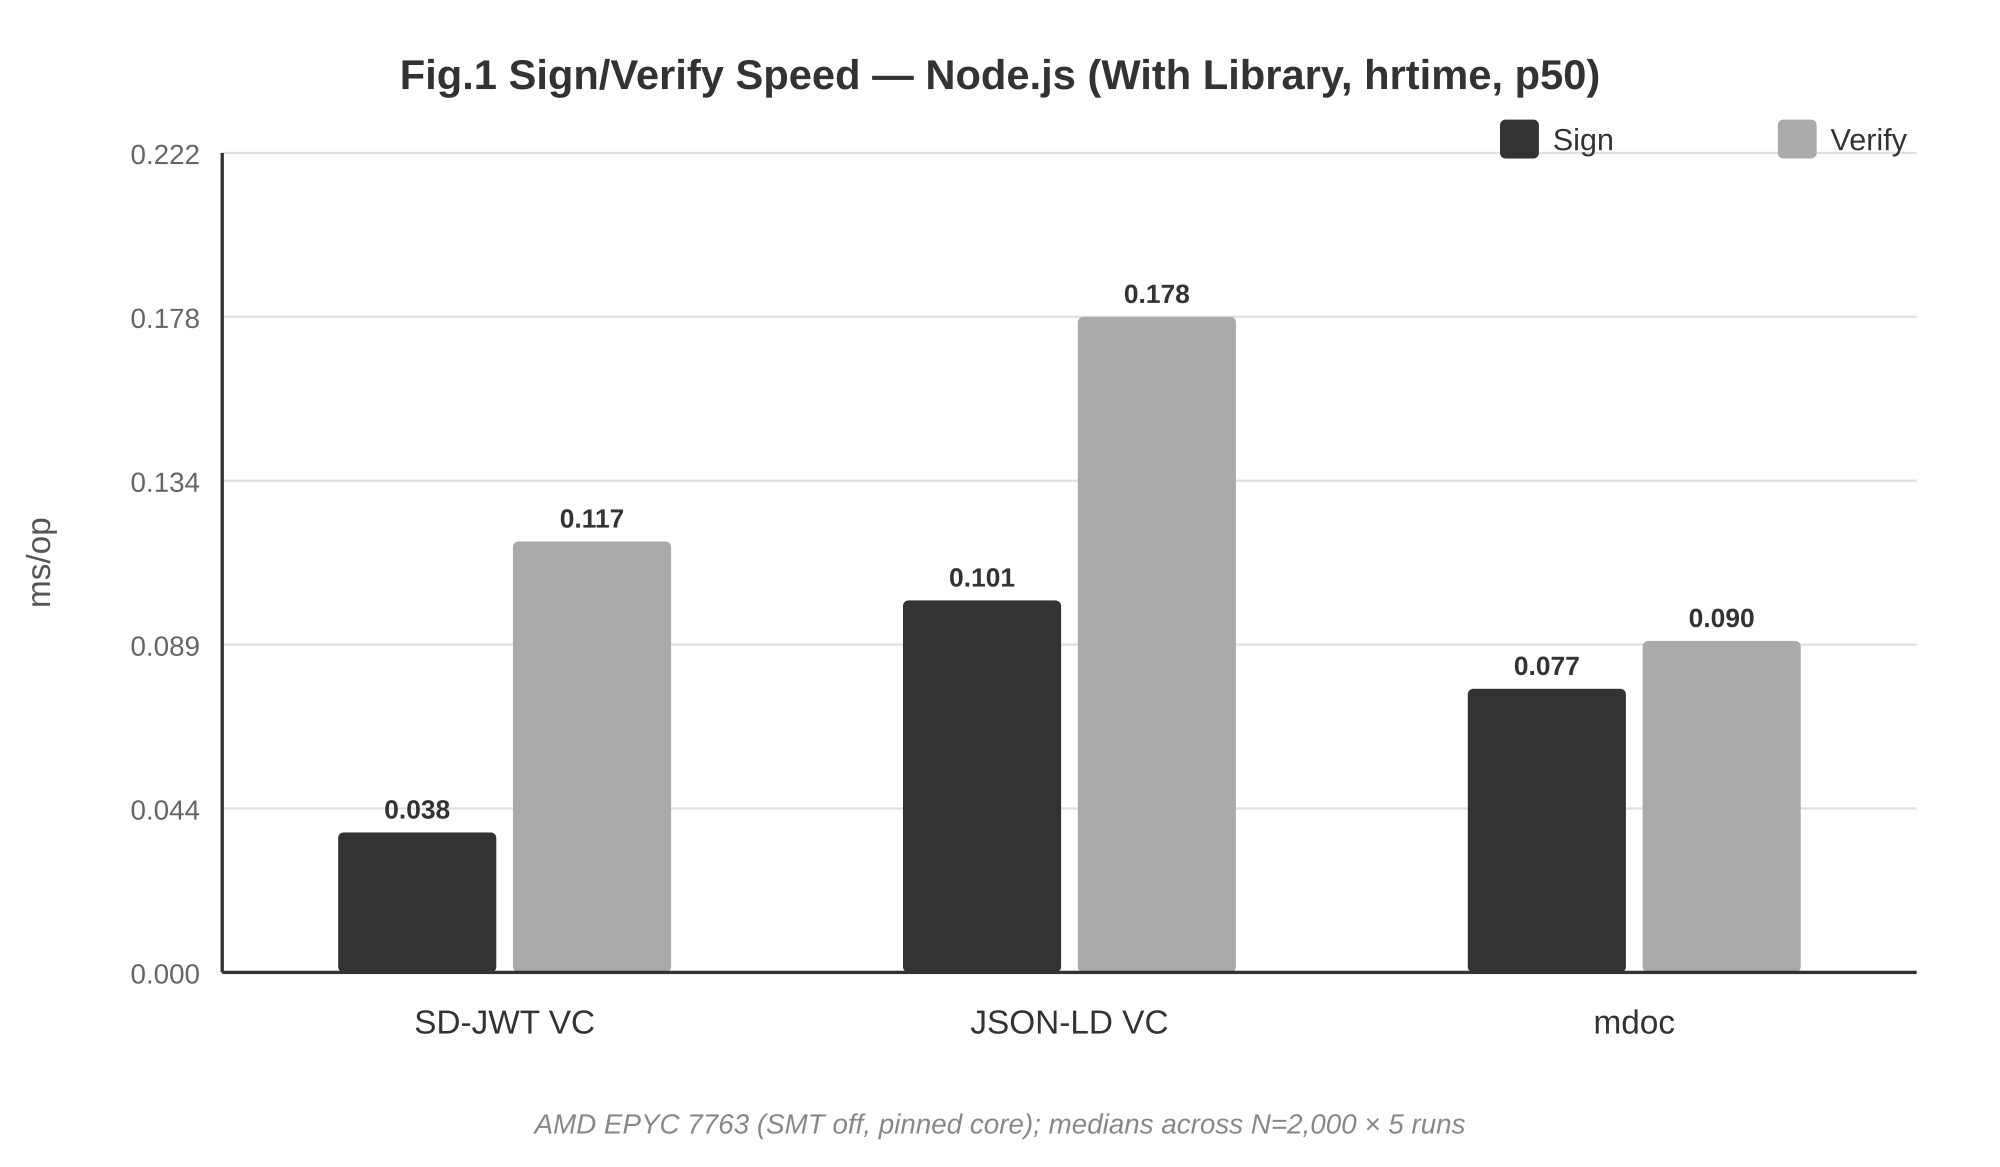
\includegraphics[width=5in,height=2.91667in]{latex/media/media/10a1a1e7bcd5189e14009557da04897e3c805595.png}

\textbf{Figure 2. Signing/Verification Speed --- Python (With Library, p50)}

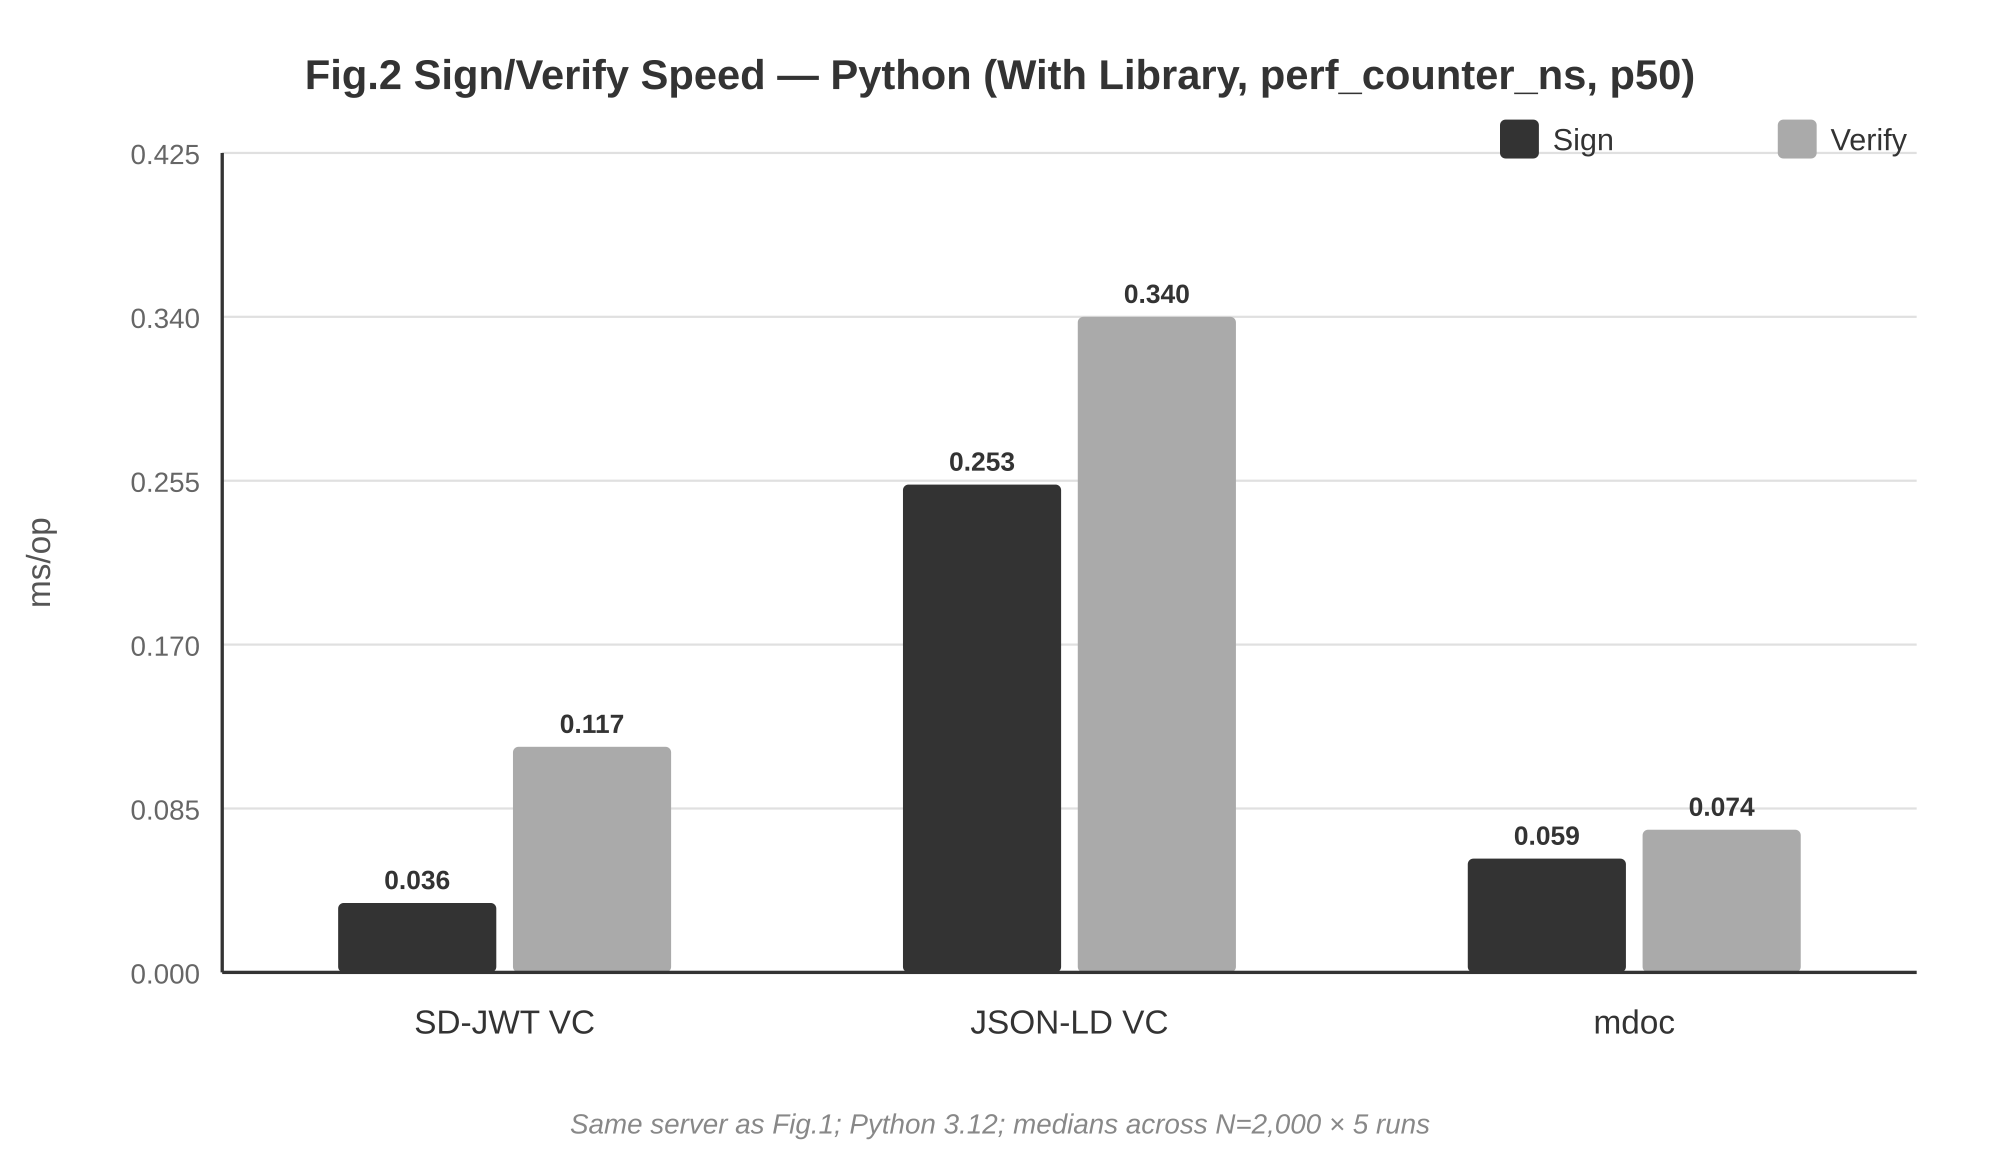
\includegraphics[width=5in,height=2.91667in]{latex/media/media/c20a2532032f14959fd98f3dde46f5b6fae5ab12.png}

\textbf{Figure 3. Signing/Verification Speed --- Go (With Library, p50)}

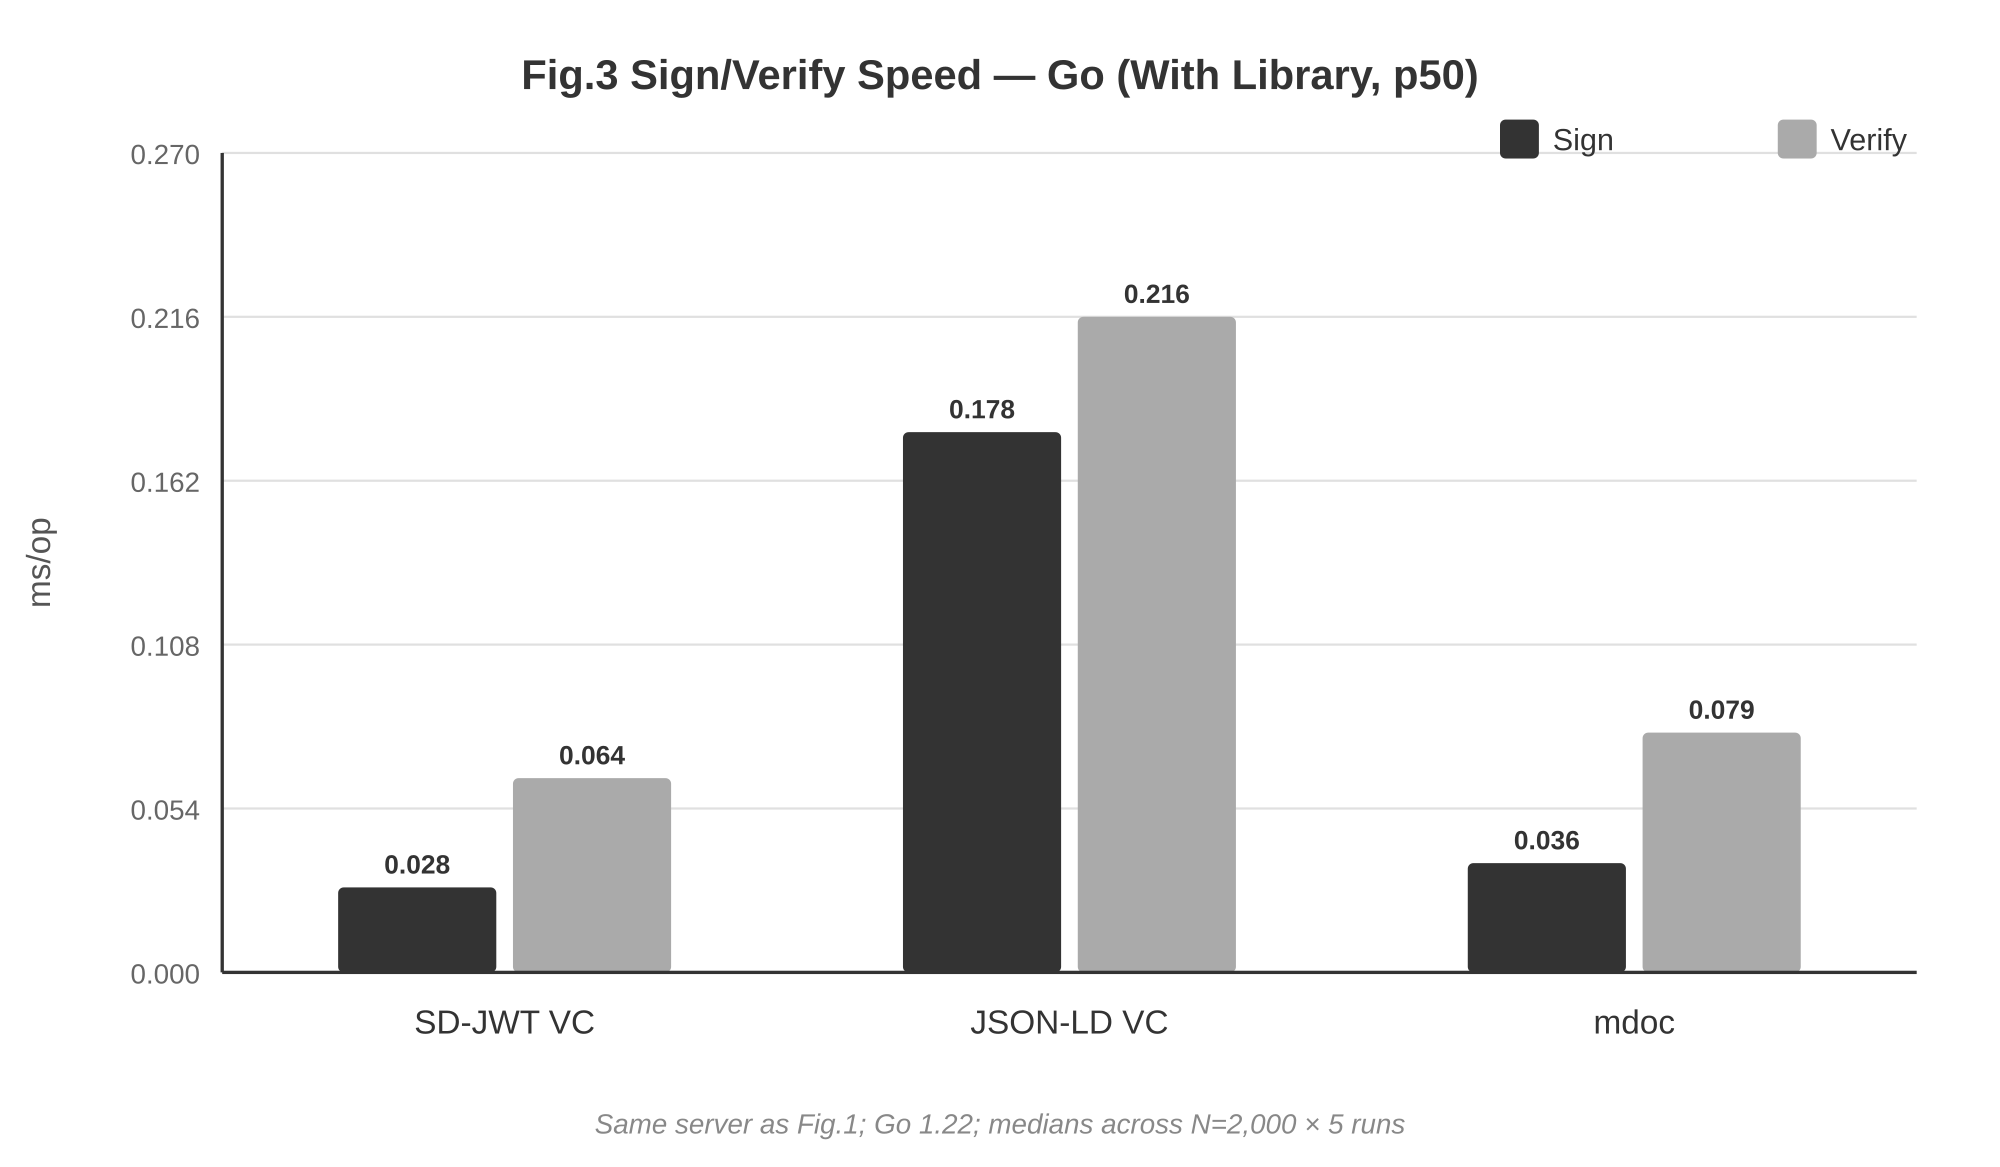
\includegraphics[width=5in,height=2.91667in]{latex/media/media/aca9e1f5edc752f3e3ae1b813c612d42c18d1c63.png}

In Node.js (Figure 1), SD-JWT VC signed fastest (0.038 ms) and mdoc verified fastest (0.090 ms). In Python (Figure 2), SD-JWT VC signed fastest (0.036 ms) and mdoc verified fastest (0.074 ms), while JSON-LD VC (PyLD) showed the largest canonicalization cost of the three languages (signing 0.253 ms, verification 0.340 ms; standalone canonicalization p50: 0.206 ms). In Go (Figure 3), SD-JWT VC signed fastest (0.028 ms), but for verification SD-JWT VC (0.064 ms) was faster than mdoc (0.079 ms) --- the opposite ordering from Node.js and Python. This is because Go's standard-library Ed25519 verification has different optimization characteristics from the OpenSSL-backed implementations (where ECDSA P-256 verification is comparatively fast), demonstrating in a single environment that the relative verification ordering of SD-JWT VC and mdoc depends on the language's cryptographic implementation. Meanwhile, across all three languages, JSON-LD VC with library (including URDNA2015 canonicalization) was consistently the slowest in both signing and verification (verify --- Node: 0.178 ms, Go: 0.216 ms, Python: 0.340 ms), confirming that URDNA2015 overhead is a specification-level characteristic rather than an artifact of any particular language implementation.

\textbf{5.5 Serialization Speed (Without Cryptographic Operations)}

Table 9 shows the pure serialization (encoding/decoding/canonicalization) speed without signature verification. This evaluates data transformation overhead excluding cryptographic processing. SD-JWT VC is evaluated for Base64URL encoding/decoding, JSON-LD VC for JSON serialization/parsing and URDNA2015 canonicalization, and mdoc for CBOR encoding/decoding.

\textbf{Table 9. Serialization Speed (without cryptographic processing; medians across N=2,000 × 5 runs)}

\begin{longtable}[]{@{}lllllllll@{}}
\toprule
\endhead
\textbf{Format} & \textbf{Operation} & \textbf{Mean(ms)} & \textbf{σ(ms)} & \textbf{95\%CI} & \textbf{p50(ms)} & \textbf{p95(ms)} & \textbf{ops/sec} & \textbf{Payload(B)}\tabularnewline
SD-JWT VC & encode & 0.004 & 0.027 & ±0.0012 & 0.002 & 0.004 & 264,594 & 322\tabularnewline
SD-JWT VC & decode & 0.005 & 0.051 & ±0.0022 & 0.003 & 0.004 & 211,999 & 322\tabularnewline
JSON-LD VC & encode & 0.002 & 0.019 & ±0.0009 & 0.001 & 0.003 & 485,827 & 464\tabularnewline
JSON-LD VC & decode & 0.002 & 0.007 & ±0.0003 & 0.002 & 0.002 & 452,419 & 464\tabularnewline
JSON-LD VC & URDNA2015 (jsonld) & 0.092 & 0.285 & ±0.0125 & 0.043 & 0.089 & 10,891 & 464\tabularnewline
JSON-LD VC (JCS) & JCS (RFC 8785) & 0.011 & 0.104 & ±0.0045 & 0.006 & 0.006 & 93,669 & 612\tabularnewline
mdoc & encode & 0.006 & 0.099 & ±0.0043 & 0.003 & 0.004 & 155,408 & 497\tabularnewline
mdoc & decode & 0.006 & 0.068 & ±0.0030 & 0.003 & 0.004 & 169,916 & 497\tabularnewline
\bottomrule
\end{longtable}

In encoding, SD-JWT VC (Base64URL) achieved p50: 0.002 ms/op, JSON-LD VC (JSON.stringify) 0.001 ms/op, and mdoc (CBOR via cbor-x) 0.003 ms/op --- all on the order of microseconds. The Payload column reports the JWT token length for SD-JWT VC, the URDNA2015-normalized N-Quads for JSON-LD VC, the JCS-canonicalized JSON for JSON-LD VC (JCS), and the CBOR-encoded bytes for mdoc.

In canonicalization processing, JSON-LD VC's URDNA2015 canonicalization (jsonld library) took p50: 0.043 ms/op (mean 0.092, 10,891 ops/sec), while JCS (JSON Canonicalization Scheme, RFC 8785) took p50: 0.006 ms/op (mean 0.011, 93,669 ops/sec), approximately 7x faster. URDNA2015 performs RDF graph canonicalization including blank node relabeling, making it computationally more expensive than JCS's key sorting and whitespace removal.

These serialization processes (p50: 0.006 ms or less, excluding URDNA2015 canonicalization) are 1-2 orders of magnitude smaller than signing/verification (Table 4: p50 0.090-0.178 ms), confirming that signing/verification speed differences are dominated by cryptographic algorithms (EdDSA vs ECDSA) and verification pipeline (canonicalization/preprocessing) differences, rather than serialization format (JSON vs CBOR) differences. Note that this URDNA2015 measurement applies to a simple credential with virtually no blank nodes; for complex credentials, canonicalization becomes the dominant cost (Section 5.11).

\textbf{5.6 Attribute Count Scaling Evaluation}

Table 11 and Figure 4 show the change in serialization speed (without cryptographic processing; JSON-LD VC includes URDNA2015 canonicalization via the jsonld library) when varying the number of attributes to 5, 20, 100, and 500. Measured with process.hrtime.bigint() at N=2,000 (N=400 for JSON-LD VC at 100+ attributes) × 5 runs.

\textbf{Table 11. Attribute Count Scaling (serialization speed vs. attribute count; medians across N=2,000 × 5 runs; †JSON-LD VC at 100/500 attributes: N=400)}

\begin{longtable}[]{@{}llllllll@{}}
\toprule
\endhead
\textbf{Format} & \textbf{Attributes} & \textbf{Mean(ms)} & \textbf{ops/sec} & \textbf{σ(ms)} & \textbf{p50(ms)} & \textbf{p95(ms)} & \textbf{Size(B)}\tabularnewline
SD-JWT VC & 5 & 0.003 & 312,515 & 0.016 & 0.002 & 0.004 & 272\tabularnewline
JSON-LD VC & 5 & 0.093 & 10,776 & 0.355 & 0.039 & 0.082 & 681\tabularnewline
JSON-LD VC (JCS) & 5 & 0.014 & 70,744 & 0.131 & 0.006 & 0.008 & 581\tabularnewline
mdoc & 5 & 0.006 & 157,485 & 0.112 & 0.002 & 0.003 & 355\tabularnewline
SD-JWT VC & 20 & 0.003 & 360,433 & 0.005 & 0.002 & 0.004 & 732\tabularnewline
JSON-LD VC & 20 & 0.118 & 8,446 & 0.300 & 0.075 & 0.110 & 1,716\tabularnewline
JSON-LD VC (JCS) & 20 & 0.011 & 89,391 & 0.006 & 0.011 & 0.011 & 926\tabularnewline
mdoc & 20 & 0.007 & 142,878 & 0.011 & 0.005 & 0.009 & 1,300\tabularnewline
SD-JWT VC & 100 & 0.008 & 129,261 & 0.007 & 0.007 & 0.010 & 3,185\tabularnewline
JSON-LD VC † & 100 & 0.277 & 3,608 & 0.061 & 0.253 & 0.419 & 7,236\tabularnewline
JSON-LD VC (JCS) & 100 & 0.039 & 25,370 & 0.007 & 0.038 & 0.042 & 2,766\tabularnewline
mdoc & 100 & 0.031 & 32,487 & 0.046 & 0.030 & 0.033 & 6,417\tabularnewline
SD-JWT VC & 500 & 0.034 & 29,607 & 0.031 & 0.032 & 0.036 & 15,452\tabularnewline
JSON-LD VC † & 500 & 1.238 & 807 & 0.146 & 1.184 & 1.446 & 34,836\tabularnewline
JSON-LD VC (JCS) & 500 & 0.184 & 5,435 & 0.048 & 0.178 & 0.192 & 11,966\tabularnewline
mdoc & 500 & 0.144 & 6,952 & 0.161 & 0.141 & 0.153 & 32,262\tabularnewline
\bottomrule
\end{longtable}

\textbf{Figure 4. Attribute Count Scaling (Serialization Speed)}

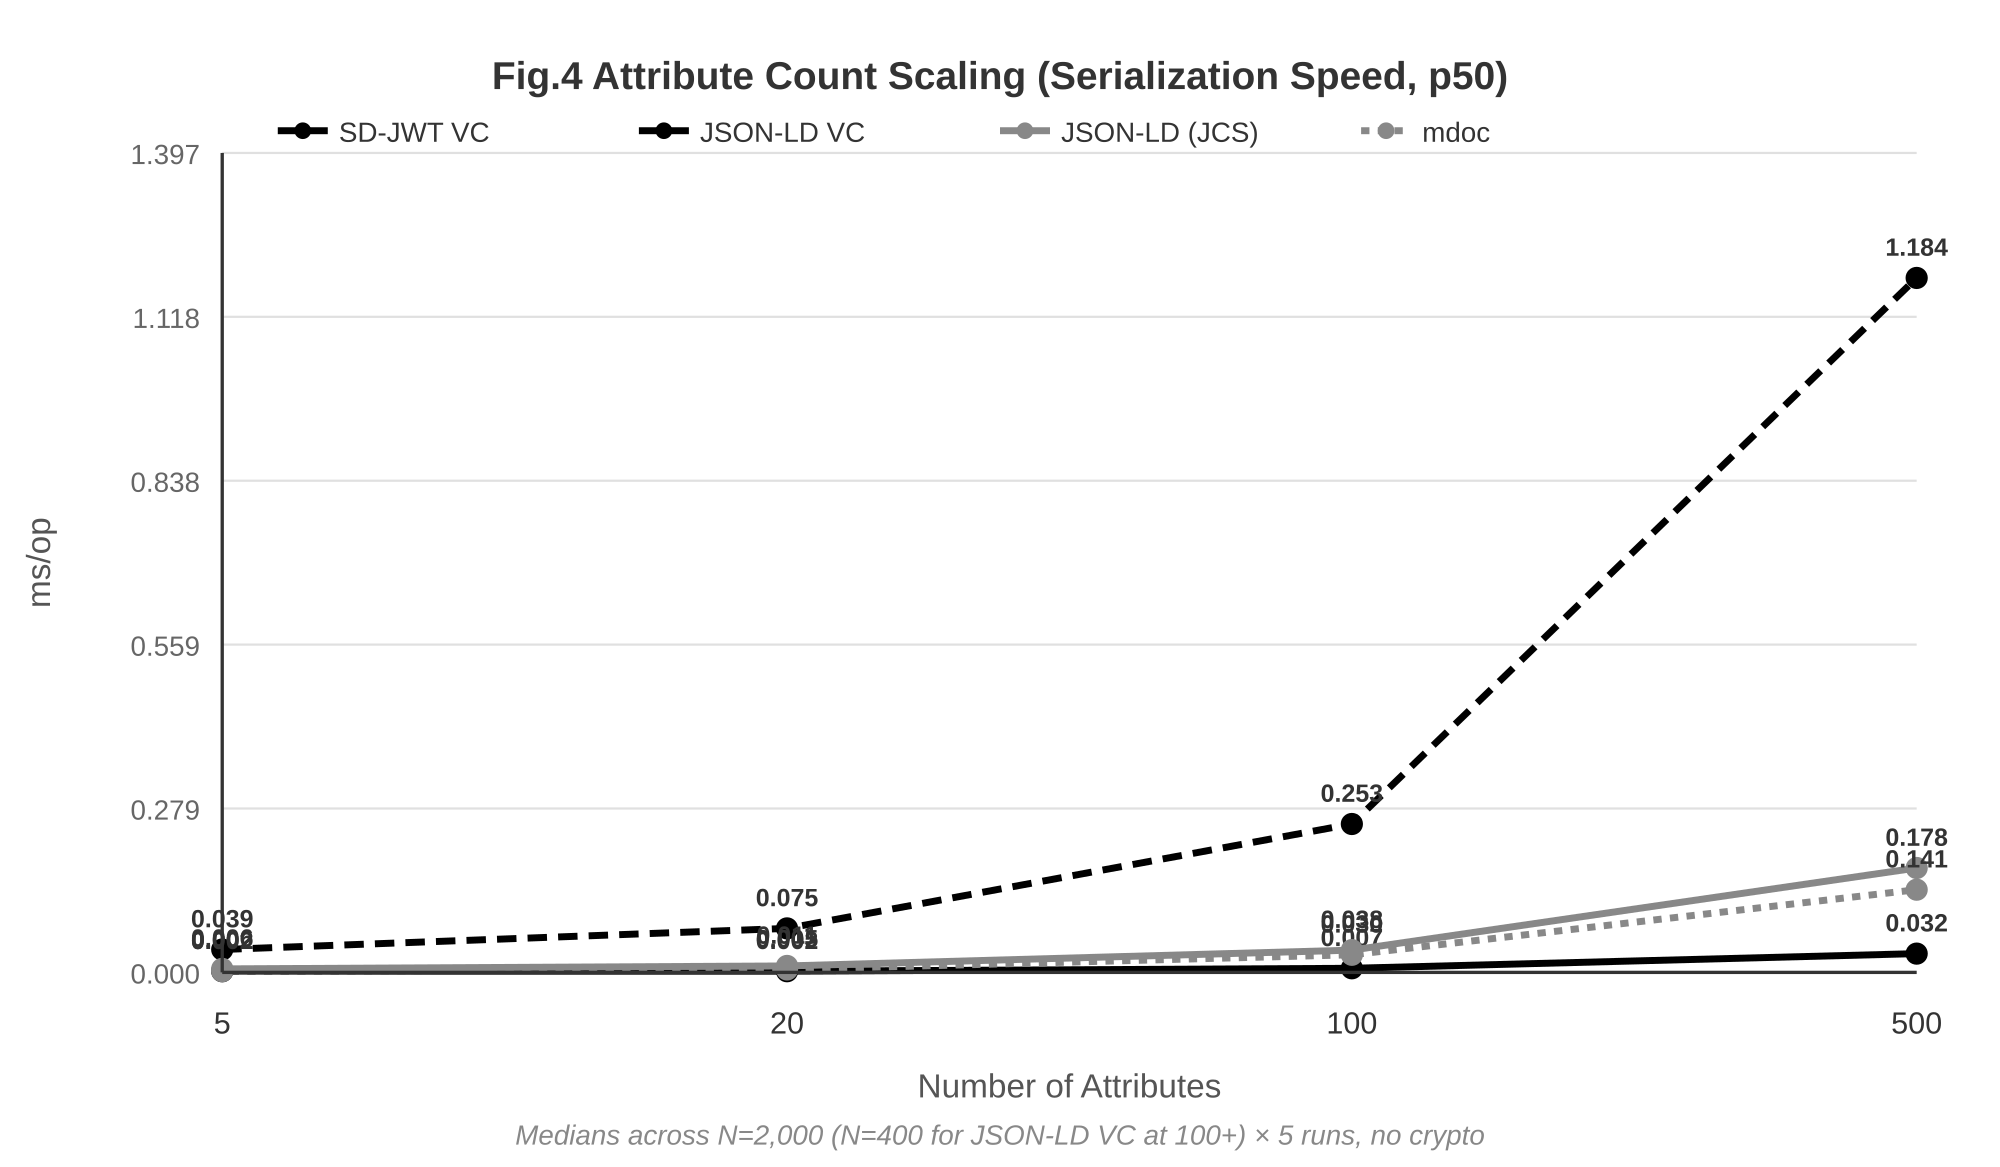
\includegraphics[width=5in,height=2.91667in]{latex/media/media/f516bf5beb9fcc2e86fd7a8be2f880b0bc042798.png}

JSON-LD VC (URDNA2015 canonicalization) serialization time showed superlinear scaling with attribute count, from p50: 0.039 ms at 5 attributes to 1.184 ms at 500 attributes (approximately 30x increase for a 100x increase in attributes; about 37x SD-JWT VC at 500 attributes). In comparison, SD-JWT VC scaling was minimal (p50: 0.002 to 0.032 ms), JCS increased from 0.006 to 0.178 ms, and mdoc from 0.002 to 0.141 ms. URDNA2015 canonicalization involves blank node relabeling and RDF dataset processing, exhibiting computational cost that increases superlinearly with the number of statements (attributes).

Regarding payload size as well, JSON-LD VC (URDNA2015-normalized N-Quads) was 34,836 bytes at 500 attributes, approximately 2.3x that of SD-JWT VC (15,452 bytes). This is because the RDF data model represents each attribute as a separate triple (subject-predicate-object), resulting in larger serialized output. mdoc was 32,262 bytes at 500 attributes, comparable to JSON-LD VC, trading readability for CBOR binary encoding.

\textbf{5.7 Selective Disclosure Performance}

Table 12 and Figure 5 show the selective disclosure (VP construction) processing speed when varying the number of disclosed attributes from 1, 3, 5, 10, to 20 out of a total of 20 attributes. Measurements use process.hrtime.bigint() (nanosecond precision) at N=2,000 × 5 runs. VP construction is a microsecond-scale operation, so resolving differences at this level requires a nanosecond-precision timer.

\textbf{Table 12. Selective Disclosure Performance Comparison (latency by number of disclosed attributes; medians across N=2,000 × 5 runs)}

\begin{longtable}[]{@{}lllllll@{}}
\toprule
\endhead
\textbf{Format} & \textbf{Disclosed} & \textbf{Mean(ms)} & \textbf{p50(ms)} & \textbf{p95(ms)} & \textbf{σ(ms)} & \textbf{Method}\tabularnewline
SD-JWT VC & 1/20 & 0.007 & 0.004 & 0.008 & 0.028 & SHA-256\tabularnewline
mdoc & 1/20 & 0.013 & 0.003 & 0.011 & 0.169 & CBOR\tabularnewline
JSON-LD VC & 1/20 & 0.003 & 0.001 & 0.002 & 0.043 & URDNA2015\tabularnewline
JSON-LD (JCS) & 1/20 & 0.006 & 0.003 & 0.003 & 0.069 & JCS\tabularnewline
SD-JWT VC & 3/20 & 0.009 & 0.004 & 0.006 & 0.147 & SHA-256\tabularnewline
mdoc & 3/20 & 0.005 & 0.003 & 0.004 & 0.042 & CBOR\tabularnewline
JSON-LD VC & 3/20 & 0.003 & 0.002 & 0.002 & 0.008 & URDNA2015\tabularnewline
JSON-LD (JCS) & 3/20 & 0.007 & 0.004 & 0.004 & 0.090 & JCS\tabularnewline
SD-JWT VC & 5/20 & 0.010 & 0.004 & 0.006 & 0.095 & SHA-256\tabularnewline
mdoc & 5/20 & 0.004 & 0.004 & 0.004 & 0.011 & CBOR\tabularnewline
JSON-LD VC & 5/20 & 0.005 & 0.003 & 0.003 & 0.066 & URDNA2015\tabularnewline
JSON-LD (JCS) & 5/20 & 0.005 & 0.004 & 0.004 & 0.021 & JCS\tabularnewline
SD-JWT VC & 10/20 & 0.005 & 0.004 & 0.005 & 0.006 & SHA-256\tabularnewline
mdoc & 10/20 & 0.005 & 0.005 & 0.005 & 0.010 & CBOR\tabularnewline
JSON-LD VC & 10/20 & 0.005 & 0.005 & 0.005 & 0.006 & URDNA2015\tabularnewline
JSON-LD (JCS) & 10/20 & 0.006 & 0.005 & 0.006 & 0.005 & JCS\tabularnewline
SD-JWT VC & 20/20 & 0.006 & 0.006 & 0.006 & 0.006 & SHA-256\tabularnewline
mdoc & 20/20 & 0.008 & 0.007 & 0.009 & 0.010 & CBOR\tabularnewline
JSON-LD VC & 20/20 & 0.009 & 0.008 & 0.009 & 0.007 & URDNA2015\tabularnewline
JSON-LD (JCS) & 20/20 & 0.009 & 0.008 & 0.009 & 0.005 & JCS\tabularnewline
\bottomrule
\end{longtable}

\textbf{Figure 5. Selective Disclosure Performance (by Number of Disclosed Attributes)}

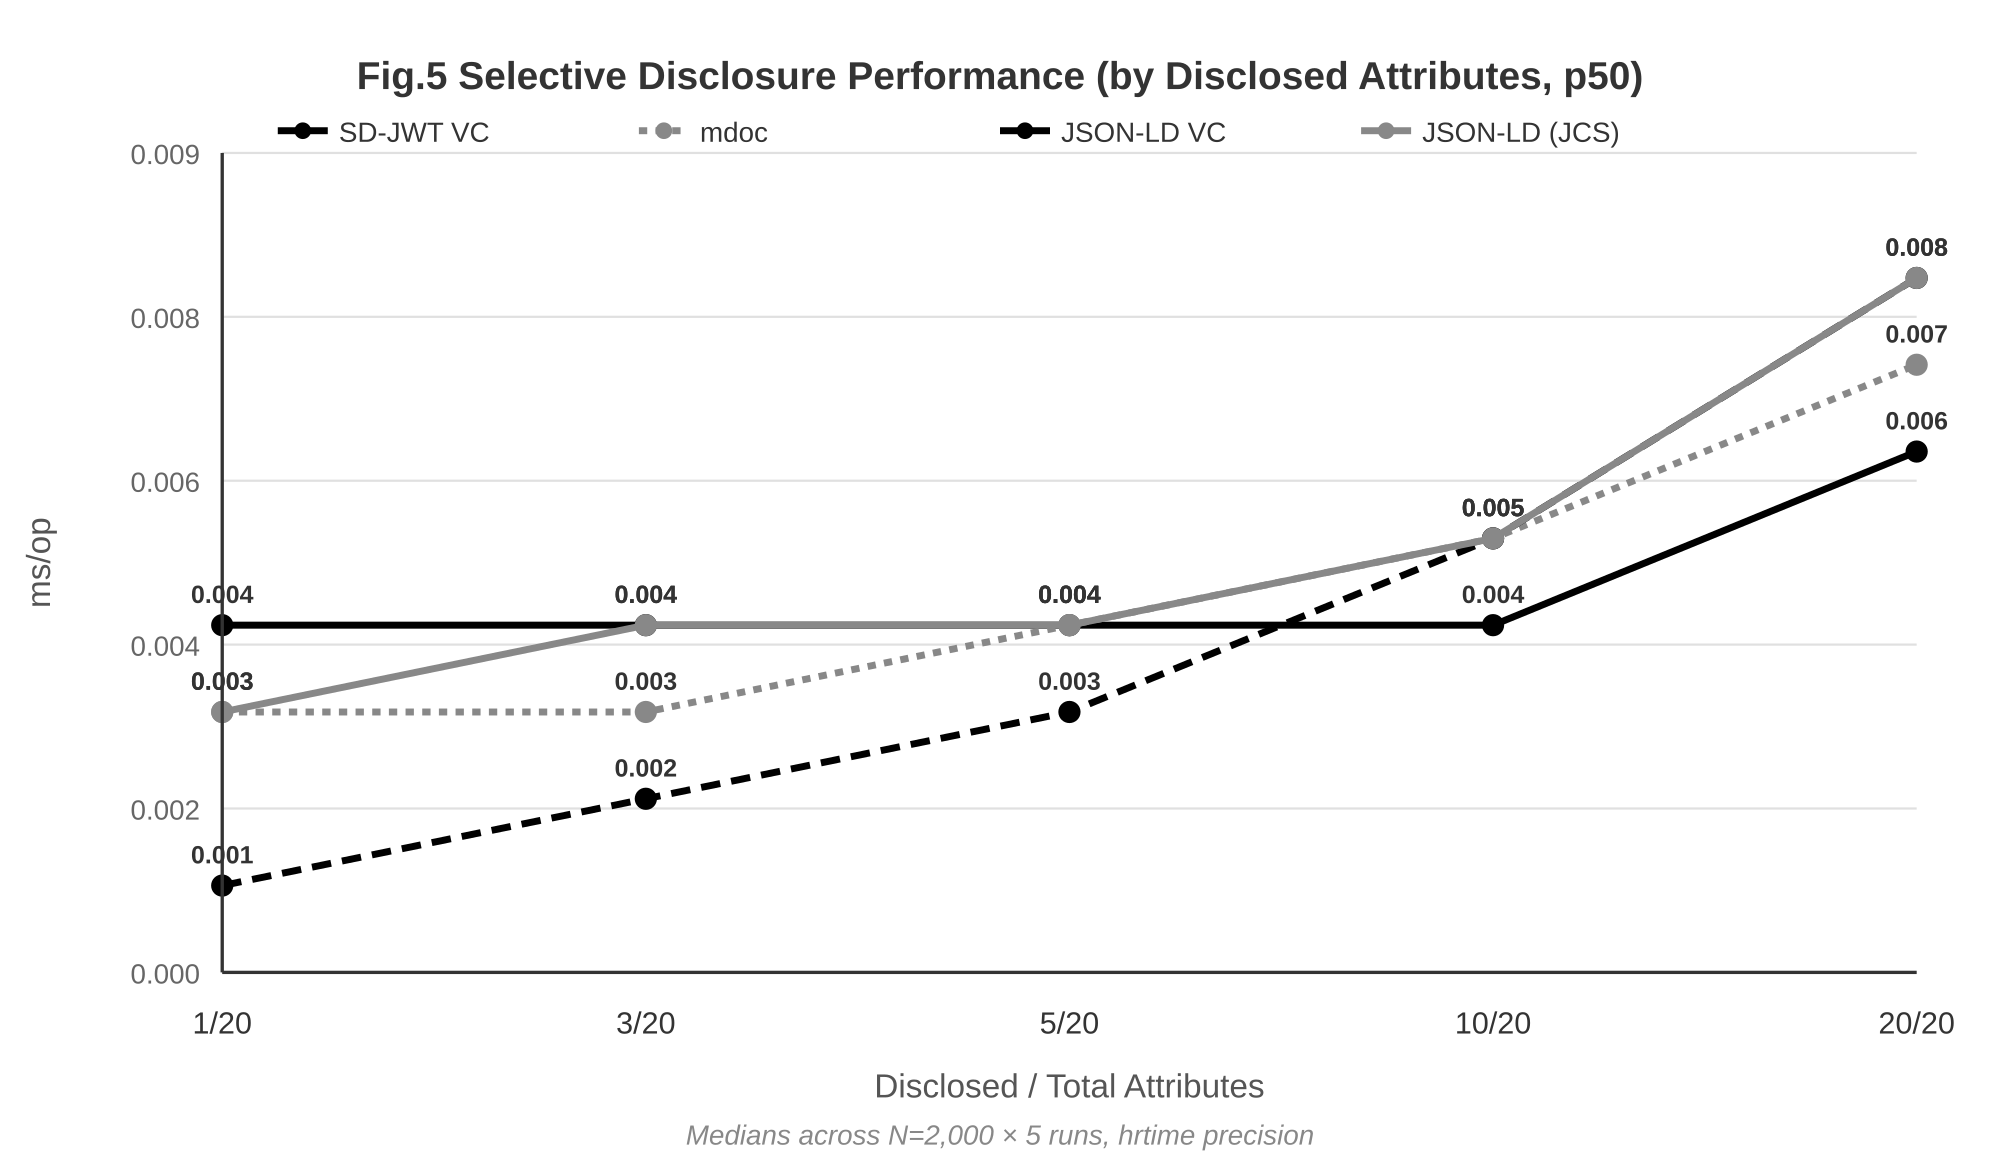
\includegraphics[width=5in,height=2.91667in]{latex/media/media/09110cf746d3bcc5047d29d6f3ed75a0c8f18145.png}

The measurements show that VP construction takes on the order of 1-8 microseconds at p50 (0.001-0.008 ms) for every format --- one to two orders of magnitude below signature verification (Table 4: p50 0.090-0.178 ms). JSON-LD VC, mdoc, and JSON-LD VC (JCS) increase monotonically with the number of disclosed attributes (JSON-LD VC: p50 0.001 ms at 1/20 to 0.008 ms at 20/20), while SD-JWT VC shows the weakest dependence on disclosure count (p50: 0.004-0.006 ms). This is because SD-JWT VC presentation only concatenates the selected disclosures, whereas the other approaches re-encode or re-canonicalize the disclosed subset. In any case, selective disclosure processing is not a dominant cost for any format.

\textbf{5.8 JSON-LD Context Loader Comparison}

Table 13 shows the performance and security differences between static loader (local cache) and remote loader (HTTP retrieval) in JSON-LD VC signature verification. The remote loader exhibited security risks including SSRF vulnerability and context injection, while the static loader mitigated these risks.

\textbf{Table 13. JSON-LD Context Loader Comparison (N=5, exploratory; browser mode of the benchmark tool)}

\begin{longtable}[]{@{}lllll@{}}
\toprule
\endhead
\textbf{Loader} & \textbf{Mean(ms)} & \textbf{p95(ms)} & \textbf{σ(ms)} & \textbf{SSRF Risk}\tabularnewline
Static Loader (restricted) & 0.06 & 0.20 & 0.080 & Safe\tabularnewline
Remote Loader (50ms delay) & 51.54 & 52.60 & 0.809 & Dangerous\tabularnewline
\bottomrule
\end{longtable}

The verification latency with remote loader was 51.54 ms, approximately 859x that of the static loader (0.06 ms). This is because network latency is directly added to verification latency. Furthermore, the remote loader generates HTTP requests to URLs specified in @context, allowing attackers to direct requests to cloud metadata endpoints (http://169.254.169.254/) or internal network addresses. The static loader eliminates these risks by resolving context locally. The remote loader latency of 51.54 ms is a single measurement and network conditions cause high variance, but it serves as reference data demonstrating the order-of-magnitude difference from the static loader.

\textbf{5.9 DoS Mitigation via URDNA2015 Call Limit}

Table 14 shows the comparison of DoS resistance with and without URDNA2015 canonicalization call limit settings. Cyclic blank node graphs were used as input.

\textbf{Table 14. Comparison With/Without URDNA2015 Call Limit}

\begin{longtable}[]{@{}llll@{}}
\toprule
\endhead
\textbf{Graph} & \textbf{Timeout} & \textbf{Duration(ms)} & \textbf{Status}\tabularnewline
2-node cyclic graph & None & 1.6 & Completed\tabularnewline
2-node cyclic graph & Yes & 0.6 & Completed\tabularnewline
4-node cyclic graph & None & 3.1 & Completed\tabularnewline
4-node cyclic graph & Yes & 0.7 & Completed\tabularnewline
6-node cyclic graph & None & 1.3 & Completed\tabularnewline
6-node cyclic graph & Yes & 1.2 & Completed\tabularnewline
8-node cyclic graph & None & 1.7 & Completed\tabularnewline
8-node cyclic graph & Yes & 1.7 & Completed\tabularnewline
\bottomrule
\end{longtable}

With small-scale cyclic graphs of 2-8 nodes, no significant DoS was reproduced. The difference in processing time between with and without call limit was small (1.1-3.3 ms), and all completed within normal processing time. However, as documented in the W3C RDFC-1.0 specification security considerations {[}9{]}, URDNA2015 canonicalization has worst-case exponential computational complexity for blank node graphs, and with several hundred or more nodes, DoS can potentially manifest. The call limit serves as a mitigation measure by aborting processing when the call count exceeds a threshold, but appropriate threshold setting requires consideration of the expected maximum blank node count in the application.

\textbf{5.10 Ed25519 Unified Algorithm Benchmark}

The main benchmark in Table 4 used Ed25519 for SD-JWT VC and JSON-LD VC and ECDSA P-256 for mdoc, so signature algorithm differences constitute a confounding factor. Table 15 shows the results of unifying all three formats under Ed25519, with the payload also unified to 5 attributes, to isolate this confound. The implementation level is identical to the with-library configuration of Table 4 (only mdoc's COSE alg changes to -8/EdDSA), measured with process.hrtime.bigint() at N=2,000 × 5 runs. Note that the mdoc Ed25519 values represent a non-standard configuration (ISO/IEC 18013-5 primarily specifies ECDSA).

\textbf{Table 15. Ed25519-Unified Benchmark (all formats with same algorithm and attribute count; medians across N=2,000 × 5 runs)}

\begin{longtable}[]{@{}lllllll@{}}
\toprule
\endhead
\textbf{Format} & \textbf{Operation} & \textbf{Mean(ms)} & \textbf{ops/sec} & \textbf{σ(ms)} & \textbf{p50(ms)} & \textbf{p95(ms)}\tabularnewline
SD-JWT VC & sign & 0.045 & 22,363 & 0.060 & 0.040 & 0.052\tabularnewline
SD-JWT VC & verify & 0.121 & 8,262 & 0.030 & 0.118 & 0.130\tabularnewline
JSON-LD VC & sign & 0.170 & 5,872 & 0.322 & 0.108 & 0.309\tabularnewline
JSON-LD VC & verify & 0.199 & 5,024 & 0.134 & 0.180 & 0.207\tabularnewline
mdoc & sign & 0.071 & 14,128 & 0.155 & 0.053 & 0.068\tabularnewline
mdoc & verify & 0.116 & 8,598 & 0.005 & 0.115 & 0.124\tabularnewline
\bottomrule
\end{longtable}

When unified under Ed25519, SD-JWT VC remained the fastest signer (p50: 0.040 ms/op), followed by mdoc (0.053 ms/op) and JSON-LD VC (0.108 ms/op). In verification, SD-JWT VC (p50: 0.118 ms/op) and mdoc (p50: 0.115 ms/op) became equivalent within measurement variation, while JSON-LD VC was approximately 1.5x (0.180 ms/op). Most notably, mdoc verification increased from p50: 0.090 ms/op with ECDSA P-256 (Table 4) to 0.115 ms/op with Ed25519 --- a 1.3x increase. For signing, conversely, mdoc with Ed25519 (0.053 ms/op) was faster than with ECDSA P-256 (0.077 ms/op). That is, the verification speed advantage of mdoc's default configuration derives partly from OpenSSL's fast ECDSA P-256 verification rather than from the CBOR/COSE structure. Meanwhile, JSON-LD VC's residual gap (\textasciitilde1.5x vs SD-JWT VC) stems from the URDNA2015 canonicalization and JSON-LD processing inherent in its verification pipeline, and does not disappear when the algorithm is unified.

\textbf{5.11 URDNA2015 Canonicalization on Complex Credentials}

Table 16 contrasts the simple credential used in the main benchmark (5 quads, virtually no blank nodes) with complex credentials based on production schemas. The evaluated credentials are: a 1EdTech Open Badges v3.0 (OB3) AchievementCredential, widely used in the education domain (containing id-less nodes such as criteria, alignment, and result); a sample modeled on the OB3-profile academic degree credentials issued by the Digital Credentials Consortium (DCC); and synthetic credentials with 10 and 50 id-less child nodes to isolate the effect of blank node count. All JSON-LD contexts are statically embedded; no network I/O is included in the measurements.

\textbf{Table 16. URDNA2015 Canonicalization of Complex Credentials (jsonld library; medians across 5 runs; N=1,000, †N=200 for OB3, DCC-style, and 50 blank nodes)}

\begin{longtable}[]{@{}llllllll@{}}
\toprule
\endhead
\textbf{Credential} & \textbf{Quads} & \textbf{Blank Nodes} & \textbf{Mean(ms)} & \textbf{σ(ms)} & \textbf{p50(ms)} & \textbf{p95(ms)} & \textbf{vs Simple (p50)}\tabularnewline
Simple (same as Table 4) & 5 & 1 & 0.088 & 0.220 & 0.049 & 0.125 & 1.0x\tabularnewline
Open Badges v3.0 & 32 & 4 & 2.449 & 2.853 & 1.992 & 4.019 & 40.7x\tabularnewline
DCC-style degree credential & 21 & 2 & 1.731 & 2.847 & 1.089 & 3.188 & 22.2x\tabularnewline
Synthetic (10 blank nodes) & 43 & 10 & 0.323 & 0.579 & 0.188 & 1.742 & 3.8x\tabularnewline
Synthetic (50 blank nodes)† & 203 & 50 & 0.770 & 0.124 & 0.751 & 0.775 & 15.3x\tabularnewline
\bottomrule
\end{longtable}

\textbf{Figure 6. URDNA2015 Canonicalization of Complex Credentials (p50)}

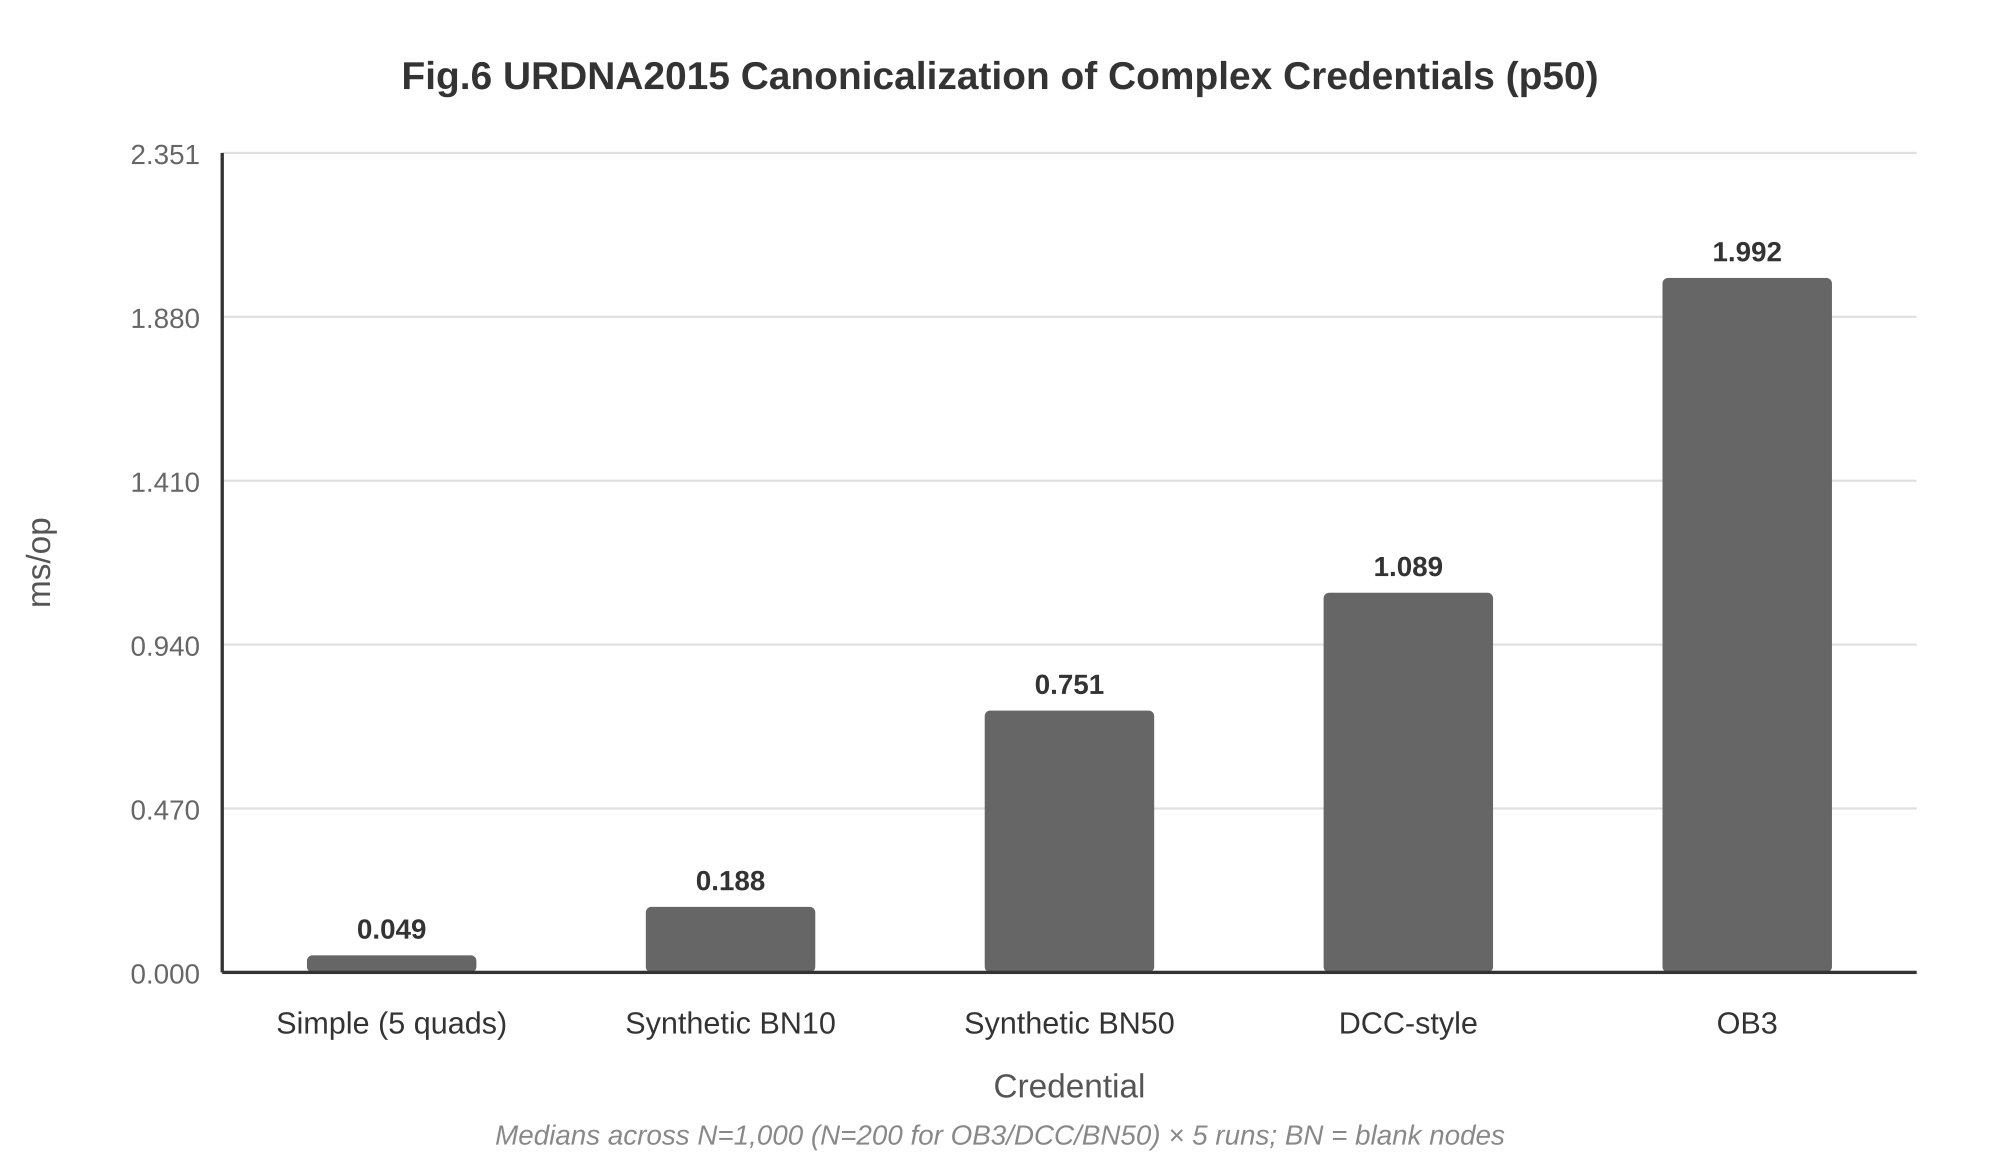
\includegraphics[width=5in,height=2.91667in]{latex/media/media/6fe8791cde7458b2b7a11496d466a5145123339c.png}

Canonicalizing the OB3 credential took p50: 1.992 ms --- roughly 41x the simple credential (0.049 ms) and more than an order of magnitude above the entire signature verification pipeline (Table 4: p50 0.090-0.178 ms). The DCC-style credential took about 22x (p50: 1.089 ms). Two factors drive this increase. First, expansion of OB3's large JSON-LD context (hundreds of term definitions) --- this explains why the cost is disproportionate to the modest quad count (32) and blank node count (4). Second, blank node canonical labeling: the synthetic credentials (10 nodes: 0.188 ms; 50 nodes: 0.751 ms) show superlinear growth in blank node count. For OB3 and DCC-style credentials, the mean-median gap and σ are also large (OB3: mean 2.449 ms with σ 2.853), indicating that complex context processing has a long latency tail.

This result shows that the observation in Section 5.1 --- that canonicalization overhead is comparatively small for simple credentials --- does not generalize to production schemas. In domains where JSON-LD VC adoption is advancing with education credentials (OB3/DCC), mitigations such as pre-compiled contexts, expansion caching, and blank node count limits become practically important. SD-JWT VC and mdoc require no canonicalization, so schema complexity has limited impact on their verification cost.

\textbf{6. Discussion}

\textbf{6.1 Discussion on Signature Verification Performance}

The structural reason SD-JWT VC achieves the fastest signing is that the adoption of JWT Compact Serialization eliminates the need for preprocessing (canonicalization) of the signing target data. The results --- signing at p50: 0.038 ms/op and verification at p50: 0.117 ms/op --- reflect the low computational cost of EdDSA (Ed25519) and the preprocessing-free structure. In the Ed25519-unified benchmark (Table 15), SD-JWT VC also signed fastest (p50: 0.040 ms/op), confirming a structural advantage for signing that is independent of algorithm (verification under a unified algorithm was equivalent to mdoc). As the reference measurements in Table 8 show, however, routing through the full JWT pipeline of the \emph{jose} library (\emph{SignJWT} / \emph{jwtVerify}, including claims validation) yields signing at 0.101 ms and verification at 0.170 ms (p50) --- 1.5-2.7x the raw cryptographic operations. Whether the structural advantage translates into production performance thus depends on the library stack in use.

From the JSON-LD VC signing breakdown (Table 5), for a simple credential URDNA2015 canonicalization accounted for about 52\% of the breakdown total and the Ed25519 signing step for about 45\% (both p50 basis) --- the same order of magnitude. That is, as long as the credential is simple (virtually no blank nodes), canonicalization overhead remains comparable to the signature operation. This observation does not generalize to complex credentials: in the evaluation with production schemas (Section 5.11, Table 16), canonicalizing an Open Badges v3.0 credential took p50: 1.992 ms --- about 41x the simple case and an order of magnitude above the entire signature verification pipeline. SHA-256 hashing (p50: 0.002 ms) is not a bottleneck.

Overall, JSON-LD VC verification latency (p50: 0.178 ms/op) is approximately 1.5x that of SD-JWT VC (p50: 0.117 ms/op). Notably, the without-library implementation of JSON-LD VC verifies at p50: 0.120 ms/op, equivalent to SD-JWT VC, demonstrating that most of the gap stems from the jsonld library's JSON-LD processing overhead. However, attribute scaling (Table 11: about 37x SD-JWT VC at 500 attributes) and the complex credential evaluation (Table 16: \textasciitilde41x for the OB3 schema) show that performance degradation with credential size and structure is a format-specific concern.

mdoc requires CBOR encoding/decoding, COSE\_Sign1 structure construction, and per-data-element SHA-256 digest computation. With signing at p50: 0.077 ms/op and verification at p50: 0.090 ms/op, it demonstrated the fastest verification speed --- about 23\% faster than SD-JWT VC (0.117 ms/op). However, in the Ed25519-unified benchmark (Table 15), mdoc verification became equivalent to SD-JWT VC, confirming that this advantage derives partly from OpenSSL's fast ECDSA P-256 verification. This interpretation is consistent with the cross-language results: in Go's standard library, Ed25519 verification (0.064 ms) is faster than ECDSA P-256 verification (0.079 ms), reversing the ordering of SD-JWT VC and mdoc (Section 5.4). For signing, by contrast, ECDSA P-256 is slower than Ed25519 (0.077 vs 0.038 ms/op), making mdoc signing about 2x SD-JWT VC.

Note that in this paper's performance comparison, Ed25519 (EdDSA) was used for SD-JWT VC and JSON-LD VC, and ECDSA P-256 was used for mdoc, so the measured results include the effect of signature algorithm differences. The Ed25519-unified experiment (Section 5.10, Table 15), which also unifies the attribute count, shows that SD-JWT VC signs fastest under the same algorithm, that SD-JWT VC and mdoc verify at comparable speed, and that JSON-LD VC remains \textasciitilde1.5x slower --- a residual gap attributable to the verification pipeline (canonicalization/preprocessing) rather than to the algorithm.

As practical implications, in use cases requiring mobile devices or high-frequency verification (e.g., mDL presentation at ticket gates), the performance advantage of SD-JWT VC and mdoc becomes significant. On the other hand, JSON-LD VC provides benefits of semantic interoperability and linked data integration in systems where these are required.

\textbf{6.2 Discussion on Implementation Complexity}

SD-JWT VC deserialization completes in approximately 10 lines, with only 3 branch points for alg allowlist, missing iss, and missing vct. The small code volume is favorable for review, auditing, and security assessment, and the single external dependency (jose) also facilitates supply chain risk management.

JSON-LD VC, with 35 lines of code, 4 asynchronous steps, and cyclomatic complexity of 8, is the most complex among the three formats. In particular, external context retrieval (2 network calls) embeds network dependency in the verification process, expanding the potential for error handling omissions and security configuration mistakes. The 2 external dependencies (jsonld, jsonld-signatures) also increase the supply chain attack surface.

mdoc shows intermediate complexity with 25 lines, 2 asynchronous steps, and cyclomatic complexity of 5. With two clearly separated processing stages of CBOR decoding and COSE\_Sign1 verification, it requires no external network calls, and the complexity is structurally manageable. The single external dependency (cbor-x) does not add network-related risk.

From a developer experience perspective, SD-JWT VC has low learning cost as signing and verification complete with a single node:crypto Ed25519 sign/verify API call. JSON-LD VC requires understanding three layers: JSON-LD processor, RDF canonicalization, and cryptographic libraries, presenting a high barrier to entry. mdoc requires understanding CBOR/COSE, but the processing flow is clear in two stages, with intermediate learning cost.

\textbf{6.3 Discussion on Security}

\textbf{6.3.1 Attack Surface of JSON-LD/RDFC Verification Pipeline}

The JSON-LD/RDFC verification pipeline has additional attack surfaces derived from remote context resolution and URDNA2015 canonicalization. This paper's experiments were conducted with default settings (no mitigations), and all three vulnerability types (poison graph DoS, context injection, SSRF) can be mitigated with appropriate production settings: static document loader, context allowlist, URDNA2015 call limit, and HTTP request timeouts. However, these mitigations require explicit configuration by developers, and the risk of vulnerability exposure due to default settings can potentially manifest.

Regarding poison graph DoS, the URDNA2015 algorithm requires worst-case exponential computational complexity in canonical labeling of blank nodes {[}9{]}. Tests confirmed that input of a poison graph composed of 20 blank nodes significantly increased processing time compared to normal credential canonicalization. Even benign production schemas already exhibit substantial cost: canonicalizing a simple credential took p50: 0.049 ms, whereas an Open Badges v3.0 credential took 1.992 ms (\textasciitilde41x, Table 16) and a synthetic credential with 50 blank nodes took 0.751 ms (\textasciitilde15x); adversarially constructed graphs can grow far worse. The W3C RDFC-1.0 specification recommends using the call limit parameter (setting an upper limit on canonicalization call count) to address this issue.\textsuperscript{1)}.

Regarding context injection, an attacker adding term definitions to JSON-LD's @context can alter the interpretation of terms like issuer and credentialSubject without invalidating the signature. This attack exploits the characteristic that JSON-LD's semantics are dynamically determined by @context. The static loader mitigates this risk by fixing context to pre-defined definitions and ignoring unknown @context URLs.

Regarding SSRF, the JSON-LD processor sends HTTP requests to URLs specified in @context. If an attacker specifies a cloud metadata endpoint (http://169.254.169.254/) or internal network address, the verifier's server makes requests to these addresses, creating a risk of internal information leakage. The static loader eliminates network access itself, completely preventing this attack vector.

\textbf{6.3.2 Security of SD-JWT VC}

In tests against SD-JWT VC, both alg:none attacks and algorithm confusion attacks were appropriately rejected by the \emph{jose}library. This indicates implementation compliance with RFC 8725 (JWT Best Current Practices) {[}5{]}. However, \emph{jose}other JWT implementations have known vulnerabilities that accept alg:none\textsuperscript{2)}, making library security track record important when selecting. Additionally, defending against algorithm confusion attacks requires explicitly specifying the algorithms option on the verification side.

\textbf{6.3.3 Security of mdoc}

mdoc correctly detected tampering in both tampering detection tests verified in this paper (data element tampering, COSE header tampering). Each data element is individually SHA-256 digested, and the digest is included in the MSO (signed by COSE\_Sign1), so even single-byte modifications are detected as digest mismatches. COSE protected header tampering is also detected because the protected header is included in the Sig\_Structure and covered by the signature. These results confirm the robustness of mdoc's data integrity protection mechanism within the scope of the evaluated attack vectors.

\textbf{6.4 Trade-off Structure of Format Characteristics}

From the comparison of the three formats, the following trade-off structure emerges. SD-JWT VC offers the fastest signing speed, simplest implementation, and mature library ecosystem, but lacks semantic expressiveness and RDF-based data integration capabilities. JSON-LD VC provides rich semantic interoperability and linked data integration, but has the most complex verification pipeline (canonicalization/preprocessing) with structural vulnerability surfaces that require explicit mitigation configuration. mdoc demonstrates the fastest verification speed with binary encoding efficiency and selective disclosure built into the data model design, but has a narrower scope of applicable use cases (physical identity documents) compared to other formats.

From the cross-language/runtime comparison (Figures 1-3, all measured on the same server) as well, the trade-off structure where JSON-LD VC with library is slowest under this paper's with-library implementation conditions was confirmed to persist across runtime environments, suggesting that URDNA2015 canonicalization overhead is an inherent characteristic at the specification level rather than an implementation or runtime-specific issue. Meanwhile, the relative verification ordering of SD-JWT VC and mdoc depends on the language's cryptographic implementation --- mdoc (ECDSA P-256) verifies faster in Node.js and Python, while SD-JWT VC (Ed25519) verifies faster in Go (Section 5.4). Additionally, the EU eIDAS 2.0 regulation {[}18{]} requires the European Digital Identity Wallet (EUDIW) to support both mdoc and SD-JWT VC formats, and the quantitative data provided by this paper can serve as a reference for implementers evaluating the performance implications of these two mandated formats.

\textbf{6.5 Use Case-Specific Recommendations}

\textbf{Table 10. Recommended Formats by Use Case}

\begin{longtable}[]{@{}lll@{}}
\toprule
\endhead
\textbf{Use Case} & \textbf{Recommended} & \textbf{Primary Reason}\tabularnewline
Web Service Authentication/Authorization & SD-JWT VC & Best performance, mature JWT ecosystem\tabularnewline
Cross-Decentralized-ID Ecosystem Interoperability & JSON-LD VC & Semantic interoperability required\tabularnewline
Mobile Identity Documents (mDL, etc.) & mdoc & ISO compliant, offline verification\tabularnewline
Education / learner credentials (Open Badges v3.0, CLR, DCC, etc.) & JSON-LD VC (OB3 profile) & 1EdTech standards and education ecosystem compatibility required; mitigations for canonicalization cost (Table 16) --- context caching, blank node limits --- are prerequisites\tabularnewline
High-throughput verification of learner credentials (e.g., bulk screening) & SD-JWT VC + OB3 vocabulary & OB3 claims carried in an SD-JWT payload verify without canonicalization; an alternative when semantic processing is unnecessary\tabularnewline
High-frequency, Low-latency Verification & SD-JWT / mdoc & No canonicalization overhead\tabularnewline
Security-first Environments & mdoc / SD-JWT & No external deps, minimal attack surface\tabularnewline
\bottomrule
\end{longtable}

As a note on the education domain: 1EdTech Open Badges v3.0 {[}19{]} and the Comprehensive Learner Record (CLR) are defined as VCDM-conformant JSON-LD VCs, and interoperability efforts such as the DCC {[}20{]} and the JFF Plugfest adopt the same profile. JSON-LD VC is therefore the de facto standard for education credentials; however, as shown in Section 5.11, the canonicalization cost of the OB3 schema reaches \textasciitilde41x that of a simple credential. Verifiers performing bulk verification (e.g., credential screening in hiring) should adopt implementation countermeasures such as statically embedded contexts and canonicalization result caching, or consider enveloping-proof (JOSE/COSE) profiles.

\textbf{7. Limitations and Future Work}

This study has several limitations. First, the measurement environment is a dedicated server with SMT disabled, unused cores taken offline, and core pinning, but it resides on a cloud VM, so hypervisor-level effects cannot be fully excluded. This paper mitigates noise by reporting medians of statistics across five independent runs, reporting outlier counts, and interpreting results primarily via p50 (run-to-run p50 variation was within 3\% for most benchmarks). JIT compilation and garbage collection effects also remain; stricter measurement on physical bare-metal hardware or with systems languages such as C/Rust is desirable.

Second, measurements with poison graphs of 20 nodes are sufficient as proof of concept, but actual DoS attacks may use several hundred to several thousand blank nodes. More extensive input is needed to verify the effectiveness of call limits under larger-scale conditions.

Third, SSRF tests statically analyzed the presence of remote URLs and did not actually send HTTP requests. Verification in real environments would require network capture within a sandbox, but this exceeds the scope of the current implementation.

Fourth, the cross-language comparison (Figures 1-3) was performed on the same server, but each language's runtime characteristics (Go: native binary, Python: interpreter with GIL, TypeScript: V8 JIT) and cryptographic library implementations (OpenSSL-backed vs. Go standard library) differ, so absolute cross-language differences should be interpreted with care; the comparison targets relative ordering and trends.

Fifth, the complex credential evaluation (Section 5.11) covers two Open Badges v3.0-family schemas and synthetic credentials; extending it to other production schemas --- multi-namespace mDL mdocs, EUDIW (eIDAS 2.0) PID/EAA schemas, and so on --- remains future work.

This paper conducted additional evaluations of attribute count scaling (Section 5.6), selective disclosure (Section 5.7), context loader comparison (Section 5.8), URDNA2015 call limit (Section 5.9), Ed25519-unified benchmark (Section 5.10), and complex credential canonicalization (Section 5.11) to more comprehensively understand the performance and security characteristics of each format. These supplementary experiments clarify the behavior of each format under conditions different from the main benchmark (Table 4), contributing to a multi-faceted understanding. Future work is expected to validate with a broader set of experimental conditions including replication on physical bare-metal hardware, large-scale blank node graphs, real mobile device measurements, and cross-network latency measurements.

\textbf{8. Threats to Validity}

We discuss threats to validity that may affect the generalizability of this paper's results.

Internal Validity: Benchmarks were measured using process.hrtime.bigint() on the Node.js V8 runtime, and V8 JIT optimization, GC pauses, and event loop interference may affect measurement stability. To mitigate this, 50 warmup iterations preceded the main N=2,000 measurements, the suite was repeated across 5 independent runs with medians of statistics reported, and outliers (Tukey 1.5×IQR) are reported without removal while p50 serves as the primary statistic. Measurements were performed on a dedicated server with SMT disabled and core pinning, but it resides on a cloud VM, so hypervisor-level effects cannot be fully excluded and hardware dependence remains (physical bare-metal replication is future work, Section 7).

Construct Validity: The benchmarks used Ed25519 for SD-JWT VC and JSON-LD VC and ECDSA P-256 for mdoc, so performance differences include the effect of signature algorithm differences. The Ed25519-unified experiment (Section 5.10) isolates this confound, showing that SD-JWT VC signs fastest independent of algorithm, that SD-JWT VC and mdoc verify at comparable speed under the same algorithm, and that mdoc's default verification advantage partly depends on ECDSA P-256 (p50: 0.115 vs 0.090 ms/op --- about 1.3x; the cross-language results in Section 5.4 corroborate this). Deserialization and verification implementation complexity metrics (LOC, cyclomatic complexity) are measured for the benchmark implementation code and may not reflect all possible implementation patterns.

External Validity: The credentials used in the main signing/verification benchmarks (Tables 4 and 8) are simple structures composed of a small number of fields such as name, date of birth, and address. Attribute count scaling for serialization speed was evaluated from 5 to 500 attributes in Section 5.6 (Table 11), and canonicalization of complex, nested schemas containing blank nodes was evaluated in Section 5.11 (Table 16) using Open Badges v3.0, DCC-style, and synthetic credentials; however, the complex schemas evaluated center on the education-domain OB3 profile, and generalization to other production schemas requires further experiments. Additionally, the benchmarks were conducted on an x86\_64 (AMD EPYC) server; results on other architectures or mobile SoCs may differ (measurements on an arm64 virtual environment during development showed absolute values roughly 2-3x faster, underscoring hardware dependence).

Security evaluation validity: Security tests against JSON-LD VC were conducted with default settings (no document loader restrictions, no call limit, no context allowlist), and risks may be mitigated in production environments with appropriate settings. The attack vectors tested are known threats documented in W3C specifications and academic literature, and do not cover zero-day vulnerabilities or novel attack techniques.

Implementation complexity validity: LOC (lines of code) heavily depends on implementation style, presence of error handling, and degree of library utilization. Cyclomatic complexity targets the entire deserialization function and may not capture internal library processing complexity. The number of external dependency libraries is a proxy indicator for supply chain risk, but does not account for individual library maturity, maintenance status, or CVE history.

\textbf{9. Conclusion}

This paper conducted a reproducible comparative evaluation of three formats---SD-JWT VC, JSON-LD VC, and mdoc---across three axes of signature verification performance, implementation complexity, and security, providing quantitative data for implementers and standardization stakeholders. The benchmark tool is published as open source {[}14{]}, enabling third-party reproducibility.

In signature verification performance, nanosecond-precision measurement on a dedicated Linux server with SMT disabled and core pinning (medians across N=2,000 × 5 runs) revealed that SD-JWT VC was fastest in signing speed (p50: 0.038 ms/op), followed by mdoc (0.077 ms/op), with JSON-LD VC at 0.101 ms/op. In verification speed, mdoc was fastest (p50: 0.090 ms/op), about 23\% faster than SD-JWT VC (0.117 ms/op), followed by JSON-LD VC (0.178 ms/op, approximately 1.5x vs SD-JWT VC). Comparing Node.js, Go, and Python on the same server demonstrated that JSON-LD VC with library is consistently the slowest across languages, while the relative verification ordering of SD-JWT VC and mdoc depends on the language's cryptographic implementation. Attribute scaling showed JSON-LD VC's URDNA2015 canonicalization growing superlinearly to about 37x SD-JWT VC at 500 attributes. Evaluation with production education schemas further showed that canonicalizing an Open Badges v3.0 credential costs about 41x a simple credential (p50: 1.992 ms), making URDNA2015 the dominant verification cost for real-world schemas. The Ed25519-unified benchmark separated algorithm effects from pipeline effects: SD-JWT VC signs fastest under a unified algorithm, SD-JWT VC and mdoc verify at comparable speed, and mdoc's default verification advantage depends partly on ECDSA P-256/COSE. In implementation complexity, SD-JWT VC was simplest (10 LOC, cyclomatic complexity 3) and JSON-LD VC was most complex (35 LOC, cyclomatic complexity 8), with mdoc intermediate (25 LOC, cyclomatic complexity 5).

From a security perspective, the JSON-LD/RDFC verification pipeline has additional attack surfaces derived from remote context resolution and URDNA2015 canonicalization, and three structural vulnerability types (poison graph DoS, context injection, SSRF) were identified. These can be mitigated with appropriate configuration (static document loader, context allowlist, call limit), but require explicit settings by developers. SD-JWT VC and mdoc detected tampering in all tested attack vectors within the scope of the evaluated attack vectors.

In format selection, the requirements of the target use case (interoperability, performance, security, regulatory compliance) should be comprehensively evaluated, and trade-offs should be explicitly accepted before making decisions. This paper does not aim to render a definitive superiority judgment among formats, but hopes to contribute as quantitative evidence for such decisions.

\textbf{Appendix A. Implementation Code}

This appendix presents the implementation code actually used for the measurements of signing and verification for each format. Listings 1, 3, 5, and 6 are excerpts from the Node.js engine of the measurement kit (linux-bench, node/bench.mjs, JavaScript/ESM), executed with Node.js v24.18.0 on the measurement server (Table 2). Each benchmark runs through the shared bench / benchAsync helper (pseudocode in Section 4.3.1), which records each iteration individually with process.hrtime.bigint() after warmup. The deserialization routines in Listings 2 and 4 are the TypeScript reference implementations analyzed in the complexity study (Section 4.3.2, Table 6).

\textbf{A.1 SD-JWT VC Signing and Verification}

As documented in Table 3, SD-JWT VC signing and verification are completed with node:crypto sign / verify calls (common to the with/without-library modes; the full jose JWT pipeline is measured separately as a reference). Listing 1 shows the implementation used for measurement, and Listing 2 the deserialization reference implementation used for the complexity analysis.

\textbf{Listing 1. SD-JWT VC Benchmark Implementation (linux-bench/node/bench.mjs)}

\begin{quote}
// linux-bench/node/bench.mjs --- SD-JWT VC (node:crypto)

async function runSdJwt() \{

const \{ privateKey, publicKey \} =

crypto.generateKeyPairSync('ed25519')

const header = b64url(Buffer.from(JSON.stringify(

\{ alg: 'EdDSA', crv: 'Ed25519' \})))

const payload = b64url(Buffer.from(JSON.stringify(\{

iss: 'https://issuer.example.com',

vct: 'identity', sub: 'did:example:holder' \})))

const sigInput = `\$\{header\}.\$\{payload\}`

// Sign: Ed25519 over the JWS Signing Input + token assembly

bench('sdjwt/stdcrypto/sign', N, () =\textgreater{} \{

const s = crypto.sign(null, Buffer.from(sigInput), privateKey)

void `\$\{sigInput\}.\$\{b64url(s)\}`

\})

// Verify: token split + Ed25519 verification

const token = `\$\{sigInput\}.` +

b64url(crypto.sign(null, Buffer.from(sigInput), privateKey))

bench('sdjwt/stdcrypto/verify', N, () =\textgreater{} \{

const p = token.split('.')

crypto.verify(null, Buffer.from(`\$\{p{[}0{]}\}.\$\{p{[}1{]}\}`),

publicKey, Buffer.from(p{[}2{]}, 'base64url'))

\})

\}
\end{quote}

\textbf{Listing 2. SD-JWT VC Deserialization Processing (reference implementation for the complexity analysis)}

\begin{quote}
async function deserializeSdJwt(

token: string, publicKey: CryptoKey

) \{

const parts = token.split('.')

if (parts.length !== 3) throw new Error('Invalid JWT')

// alg allowlist verification

const header = JSON.parse(atob(parts{[}0{]}))

if (!{[}'ES256','ES384','EdDSA','RS256'{]}.includes(header.alg))

throw new Error('Unsupported algorithm')

// Signature verification + claim retrieval (1 API call)

const \{ payload \} = await jwtVerify(token, publicKey)

// Required claims check

if (!payload.iss) throw new Error('Missing issuer')

if (!payload.vct) throw new Error('Missing vct')

return payload

\}
\end{quote}

\textbf{A.2 JSON-LD VC Signing and Verification}

The signing process for JSON-LD VC consists of three stages: URDNA2015 canonicalization, SHA-256 hashing, and Ed25519 signing. Listing 3 shows the implementation used for measurement: the jsonld library performs canonicalization, and node:crypto performs hashing and signing. The breakdown in Table 5 was obtained by measuring each stage individually (canonicalization only, hashing only, signing only) with the same bench helper.

\textbf{Listing 3. JSON-LD VC Benchmark Implementation (linux-bench/node/bench.mjs)}

\begin{quote}
// linux-bench/node/bench.mjs --- JSON-LD VC (jsonld + node:crypto)

async function runJsonLd() \{

const jsonld = (await import('jsonld')).default

const \{ privateKey \} = crypto.generateKeyPairSync('ed25519')

const publicKey = crypto.createPublicKey(privateKey)

const normalize = () =\textgreater{} jsonld.normalize(VC\_DOC, \{

algorithm: 'URDNA2015',

format: 'application/n-quads', safe: false \})

// Sign: URDNA2015 canonicalize -\textgreater{} SHA-256 -\textgreater{} Ed25519 sign

await benchAsync('jsonld/jsonld-lib/sign', N, async () =\textgreater{} \{

const norm = await normalize()

crypto.sign(null,

crypto.createHash('sha256').update(norm).digest(),

privateKey)

\})

// Verify: re-canonicalize -\textgreater{} SHA-256 -\textgreater{} Ed25519 verify

const sig0 = crypto.sign(null, crypto.createHash('sha256')

.update(await normalize()).digest(), privateKey)

await benchAsync('jsonld/jsonld-lib/verify', N, async () =\textgreater{} \{

const norm = await normalize()

crypto.verify(null,

crypto.createHash('sha256').update(norm).digest(),

publicKey, sig0)

\})

// Canonicalization only (Tables 5 and 9)

await benchAsync('jsonld/jsonld-lib/normalize-only', N,

async () =\textgreater{} \{ await normalize() \})

\}
\end{quote}

\textbf{Listing 4. JSON-LD VC Deserialization Processing (reference implementation for the complexity analysis)}

\begin{quote}
async function deserializeJsonLdVc(

document: Record\textless string, unknown\textgreater,

signature: Uint8Array, publicKey: Uint8Array

) \{

const loader = makeStaticContextLoader()

// 1. @context verification

const ctx = document{[}'@context'{]} as string{[}{]}

if (!ctx.includes(VC\_CONTEXT\_URL))

throw new Error('Missing VC context')

// 2. Remove proof field

const \{ proof, ...docWithoutProof \} = document

// 3. JSON-LD expansion (network retrieval occurs)

await jsonld.expand(docWithoutProof,

\{ documentLoader: loader, safe: false \})

// 4. URDNA2015 RDF canonicalization

// Blank node identification = graph isomorphism problem

const normalized = await jsonld.normalize(

docWithoutProof, \{

algorithm: 'URDNA2015',

format: 'application/n-quads',

documentLoader: loader, safe: false

\}) as string

// 5. SHA-256 hash

const hash = await sha256(normalized)

// 6. Ed25519 signature verification

const valid = await ed25519Verify(

signature, hash, publicKey)

if (!valid) throw new Error('Signature failed')

// 7. VC schema verification

if (!document{[}'credentialSubject'{]})

throw new Error('Missing credentialSubject')

return document

\}
\end{quote}

\textbf{A.3 mdoc (ISO 18013-5) Signing and Verification}

The mdoc measurement implementation consists of CBOR encoding with cbor-x, MSO construction from per-data-element SHA-256 digests, and ECDSA P-256 signing over the COSE\_Sign1 Sig\_structure (raw r\textbar\textbar s as used by COSE, dsaEncoding: ieee-p1363). Listing 5 shows the signing side and Listing 6 the verification side of the measurement implementation. For the full deserialization reference implementation including per-element digest matching, see the complexity-analysis code (Listing 11 in A.5).

\textbf{Listing 5. mdoc Signing-side Measurement Implementation (linux-bench/node/bench.mjs)}

\begin{quote}
// linux-bench/node/bench.mjs --- mdoc (cbor-x + node:crypto)

const \{ encode: cborEncode \} = await import('cbor-x')

const \{ privateKey, publicKey \} =

crypto.generateKeyPairSync('ec', \{ namedCurve: 'P-256' \})

// Build the MSO from per-IssuerSignedItem SHA-256 digests and

// produce the COSE\_Sign1 Sig\_structure

const buildSigStruct = () =\textgreater{} \{

const digestMap = new Map()

let id = 0

for (const {[}k, v{]} of MDOC\_FIELDS) \{

const item = cborEncode(\{ digestID: id,

elementIdentifier: k, elementValue: v \})

digestMap.set(id++, new Uint8Array(

crypto.createHash('sha256').update(item).digest()))

\}

const protHdr = cborEncode(new Map({[}{[}1, -7{]}{]})) // alg: ES256

const msoPayload = cborEncode(\{

docType: 'org.iso.18013.5.1.mDL',

valueDigests: digestMap \})

return cborEncode({[}'Signature1', protHdr,

new Uint8Array(0), msoPayload{]})

\}

// Sign: Sig\_structure build + ECDSA P-256 (raw r\textbar\textbar s)

bench('mdoc/cbor-x/sign', N, () =\textgreater{} \{

crypto.sign('SHA256', buildSigStruct(),

\{ key: privateKey, dsaEncoding: 'ieee-p1363' \})

\})
\end{quote}

\textbf{Listing 6. mdoc Verification-side Measurement Implementation (linux-bench/node/bench.mjs)}

\begin{quote}
// Verify: ECDSA P-256 verification of the COSE\_Sign1 signature

const ss0 = buildSigStruct()

const sig0 = crypto.sign('SHA256', ss0,

\{ key: privateKey, dsaEncoding: 'ieee-p1363' \})

bench('mdoc/cbor-x/verify', N, () =\textgreater{} \{

crypto.verify('SHA256', ss0,

\{ key: publicKey, dsaEncoding: 'ieee-p1363' \}, sig0)

\})
\end{quote}

\textbf{A.4 Security Test Implementation Examples}

The security tests (Section 4.3.4) were performed with the TypeScript implementation of the benchmark tool (VC Comparison Tool). As representative implementations, we present poison graph generation (Listing 7) and the mdoc data tampering detection test (Listing 8). These are qualitative evaluations of attack success and behavior, independent of the performance measurements (linux-bench).

\textbf{Listing 7. Poison Graph DoS Test (normalizationSecurity.ts)}

\begin{quote}
function buildPoisonGraph(depth: number) \{

const nodes: Record\textless string, unknown\textgreater{[}{]} = {[}{]}

for (let i = 0; i \textless{} depth; i++) \{

nodes.push(\{

'@type': 'http://example.org/Node',

'http://example.org/link':

\{ '@id': `\_:b\$\{(i + 1) \% depth\}` \}

\})

nodes.push(\{

'@type': 'http://example.org/Node',

'http://example.org/link':

\{ '@id': `\_:b\$\{i\}` \}

\})

\}

return \{ '@graph': nodes \}

\}

async function poisonGraphTest() \{

// Baseline: simple credential normalization

const t0 = performance.now()

await jsonld.normalize(normalDoc, normalizeOpts)

const normalMs = performance.now() - t0

// Poison: 20-node cyclic blank node graph

const poisonDoc = buildPoisonGraph(20)

const t1 = performance.now()

try \{

await jsonld.normalize(poisonDoc, normalizeOpts)

\} catch \{\}

const poisonMs = performance.now() - t1

return \{ normalMs, poisonMs,

ratio: poisonMs / Math.max(normalMs, 0.1) \}

\}
\end{quote}

\textbf{Listing 8. mdoc Data Element Tampering Detection Test (normalizationSecurity.ts)}

\begin{quote}
async function mdocCborMalleabilityTest() \{

const \{ privateKey, publicKey \} =

await generateMdocKeyPair()

const mdocBytes = await issueMdoc(

MDOC\_FIELDS, privateKey)

// Tamper: modify element value

// without updating digest

const doc = decode(mdocBytes)

const items = doc.issuerSigned

.nameSpaces{[}'org.iso.18013.5.1'{]}

const originalItem = decode(items{[}0{]})

const tamperedItem =

\{ ...originalItem, elementValue: 'ATTACKER' \}

items{[}0{]} = encode(tamperedItem)

const tamperedMdoc = encode(doc)

// Verify: should detect digest mismatch

const valid = await verifyMdoc(

tamperedMdoc, publicKey).catch(() =\textgreater{} false)

return \{ caught: !valid \}

\}
\end{quote}

\textbf{A.5 Code Analyzed in the Complexity Study (Annotated)}

This section lists the deserialization reference implementations that the complexity metrics in Section 5.2 (Table 6) were computed on. The branch, asynchronous-step, and network annotations in the comments correspond to the metrics in Table 6.

\textbf{Listing 9. SD-JWT VC Deserialization --- With Complexity Annotations}

\begin{quote}
// SD-JWT VC deserialization (\textasciitilde10 LOC)

// External deps: jose (1)

// Network calls: 0

async function deserializeSdJwt(

token: string, publicKey: CryptoKey

) \{

// -\/-\/- Preprocessing: Split JWT compact representation -\/-\/-

const parts = token.split('.')

if (parts.length !== 3) // ★Branch 1

throw new Error('Invalid JWT format')

// -\/-\/- Header verification -\/-\/-

const header = JSON.parse(

atob(parts{[}0{]}.replace(/-/g,'+').replace(/\_/g,'/')))

if (!{[}'ES256','ES384','EdDSA','RS256'{]}

.includes(header.alg)) // ★Branch 2

throw new Error('Unsupported algorithm')

// -\/-\/- Signature verification (only async step) -\/-\/-

const \{ payload \} =

await jwtVerify(token, publicKey) // ★async 1

// -\/-\/- Required claims check -\/-\/-

if (!payload.iss) // ★Branch 3a

throw new Error('Missing issuer')

if (!payload.vct) // ★Branch 3b

throw new Error('Missing vct claim')

return payload

\}
\end{quote}

\textbf{Listing 10. JSON-LD VC Deserialization --- With Complexity Annotations}

\begin{quote}
// JSON-LD VC deserialization (\textasciitilde35 LOC)

// External deps: jsonld, DocumentLoader, sha256,

// ed25519 (4)

// Network calls: 2

async function deserializeJsonLdVc(

document: Record\textless string, unknown\textgreater,

signature: Uint8Array,

publicKey: Uint8Array

) \{

// -\/-\/- Document Loader construction -\/-\/-

// ★SSRF RISK: allowlist required in production

const loader = makeStaticContextLoader()

// -\/-\/- 1. @context verification -\/-\/-

const ctx = document{[}'@context'{]} as string{[}{]}

if (!ctx \textbar\textbar{} // ★Branch 1

!ctx.includes(VC\_CONTEXT\_URL))// ★Branch 2

throw new Error('Missing VC context')

// -\/-\/- 2. Separate proof field -\/-\/-

const \{ proof: \_proof,

...documentWithoutProof \} = document

// -\/-\/- 3. JSON-LD expansion -\/-\/-

// ★NETWORK 1: Context URL retrieval

await jsonld.expand( // ★async 1

documentWithoutProof,

\{ documentLoader: loader,

safe: false \})

// -\/-\/- 4. URDNA2015 RDF canonicalization -\/-\/-

// ★DoS RISK: Blank node identification =

// graph isomorphism -\textgreater{} worst-case exponential

// ★NETWORK 2: Additional context retrieval

const normalized =

await jsonld.normalize( // ★async 2

documentWithoutProof, \{

algorithm: 'URDNA2015',

format: 'application/n-quads',

documentLoader: loader,

safe: false,

\}) as string

if (!normalized) // ★Branch 3

throw new Error('Empty normalization')

// -\/-\/- 5. SHA-256 hash -\/-\/-

const hash =

await sha256(normalized) // ★async 3

// -\/-\/- 6. Ed25519 signature verification -\/-\/-

const valid = await ed25519Verify(// ★async 4

signature, hash, publicKey)

if (!valid) // ★Branch 4

throw new Error('Signature failed')

// -\/-\/- 7. VC schema verification -\/-\/-

if (!document.type) // ★Branch 5

throw new Error('Missing type')

if (!document.issuer) // ★Branch 6

throw new Error('Missing issuer')

if (!document.credentialSubject) // ★Branch 7

throw new Error('Missing subject')

if (!document.issuanceDate) // ★Branch 8

throw new Error('Missing issuanceDate')

return document

\}
\end{quote}

\textbf{Listing 11. mdoc Deserialization --- With Complexity Annotations}

\begin{quote}
// mdoc deserialization (\textasciitilde25 LOC)

// External deps: cbor-x, WebCrypto (2)

// Network calls: 0

export async function verifyMdoc(

mdocBytes: Uint8Array,

publicKey: CryptoKey

): Promise\textless boolean\textgreater{} \{

// -\/-\/- 1. CBOR decode -\/-\/-

const doc = decode(mdocBytes)

if (!doc?.issuerSigned) // ★Branch 1

throw new Error('Invalid mdoc')

const \{ issuerAuth, nameSpaces \}

= doc.issuerSigned

const {[}protectedHeader, ,

msoPayload, signature{]} = issuerAuth

// -\/-\/- 2. COSE algorithm verification -\/-\/-

const alg = decode(protectedHeader).get(1)

if (alg !== -7) // ★Branch 2

throw new Error('Unexpected alg')

// -\/-\/- 3. COSE\_Sign1 signature verification -\/-\/-

const sigStructure = buildSigStructure(

protectedHeader, msoPayload)

const valid =

await crypto.subtle.verify( // ★async 1

\{ name: 'ECDSA', hash: 'SHA-256' \},

publicKey, signature, sigStructure)

if (!valid) // ★Branch 3

return false

// -\/-\/- 4. MSO decode + digest verification -\/-\/-

const mso = decode(msoPayload)

const storedDigests =

mso.valueDigests{[}'org.iso.18013.5.1'{]}

const items =

nameSpaces{[}'org.iso.18013.5.1'{]}

for (let i = 0; i \textless{} items.length; i++) \{

const computed = new Uint8Array(

await crypto.subtle.digest( // ★async 2

'SHA-256', items{[}i{]}))

const expected = storedDigests{[}i{]}

if (expected.length !== // ★Branch 4

computed.length) return false

for (let j = 0; j \textless{} computed.length; j++)

if (computed{[}j{]} !== // ★Branch 5

expected{[}j{]}) return false

\}

return true

\}
\end{quote}

\textbf{References}

{[}1{]} D. Fett, K. Yasuda, and B. Campbell, "SD-JWT-based Verifiable Credentials (SD-JWT VC)," IETF RFC 9901, 2024.

{[}2{]} M. Sporny, D. Longley, and D. Chadwick, "Verifiable Credentials Data Model v2.0," W3C Recommendation, 2024.

{[}3{]} ISO/IEC 18013-5:2021, "Personal identification --- ISO-compliant driving licence --- Part 5: Mobile driving licence (mDL) application," 2021.

{[}4{]} D. Longley and M. Sporny, "RDF Dataset Canonicalization (RDFC-1.0)," W3C Recommendation, 2024.

{[}5{]} Y. Sheffer, D. Hardt, and M. Jones, "JSON Web Token Best Current Practices," IETF RFC 8725, 2020.

{[}6{]} J. Schaad, "CBOR Object Signing and Encryption (COSE): Structures and Process," IETF RFC 9052, 2022.

{[}7{]} D. Fett, B. Campbell, J. Bradley, T. Lodderstedt, M. Jones, and D. Waite, "Selective Disclosure for JWTs (SD-JWT)," IETF RFC 9449, 2024.

{[}8{]} T. McLaughlin, "CVE-2015-9235: `None' Algorithm Vulnerability in JWT Libraries," NVD, 2015.

{[}9{]} W3C, "RDF Dataset Canonicalization --- Security Considerations," in RDF Dataset Canonicalization (RDFC-1.0), §4.8, W3C Recommendation, 2024. {[}Online{]}. Available: https://www.w3.org/TR/rdf-canon/\#security-considerations

{[}10{]} D. Longley, M. Sporny, and G. Kellogg, "Data Integrity 1.0," W3C Working Draft, 2024.

{[}11{]} M. Jones, J. Bradley, and N. Sakimura, "JSON Web Token (JWT)," IETF RFC 7519, 2015.

{[}12{]} C. Bormann and P. Hoffman, "Concise Binary Object Representation (CBOR)," IETF RFC 8949, 2020.

{[}13{]} D. Temoshok, D. Proud-Madruga, Y.-Y. Choong, R. Galluzzo, S. Gupta, C. LaSalle, N. Lefkovitz, and A. Regenscheid, "Digital Identity Guidelines," NIST SP 800-63-4, 2025.

{[}14{]} N. Fujie, "VC Format Comparison Tool," GitHub, 2024--2026. {[}Online{]}. Available: https://github.com/fujie/vcformatcomparison

{[}15{]} A. Buldini, C. Mazzocca, R. Montanari, and S. Uluagac, "Compact and Selective Disclosure for Verifiable Credentials," arXiv:2506.00262, 2025.

{[}16{]} S. Abraham, S. More, et al., "DID and VC: Untangling Decentralized Identifiers and Verifiable Credentials for the Web of Trust," in Proc. ACM CODASPY, 2021, pp. 169--180.

{[}17{]} A. Helm, T. Lodderstedt, and K. Yasuda, "Selective-Disclosure in Decentralised Identity: A Comparative Evaluation of BBS+ and SD-JWT," TechRxiv, 2025.

{[}18{]} European Parliament, "Regulation (EU) 2024/1183 amending Regulation (EU) No 910/2014 as regards establishing the European Digital Identity Framework (eIDAS 2.0)," Official Journal of the European Union, 2024.

{[}19{]} 1EdTech Consortium, "Open Badges Specification v3.0," 1EdTech Final Release, 2024. {[}Online{]}. Available: https://www.imsglobal.org/spec/ob/v3p0/

{[}20{]} Digital Credentials Consortium, "Digital Credentials Consortium --- Building the digital credential infrastructure for the future," MIT, 2024. {[}Online{]}. Available: https://digitalcredentials.mit.edu/
